\documentclass[UTF8,openany,oneside]{ctexbook}
\usepackage[a4paper,left=3.0cm,right=2.5cm,top=2.8cm,bottom=2.6cm,headheight=15pt,headsep=0.8cm]{geometry}
\usepackage{graphicx}
\usepackage{amsmath,amssymb}
\usepackage{booktabs}
\usepackage{array}
\usepackage{tabularx}
\usepackage{longtable}
\usepackage{enumitem}
\usepackage{caption}
\usepackage{tocloft}
\usepackage{float}
\usepackage{hyperref}
\usepackage{xurl}
\usepackage{setspace}
\usepackage{fancyhdr}
\usepackage{titlesec}
\usepackage{indentfirst}

\newcommand{\thesisschool}{请填写学校名称}
\newcommand{\thesistype}{本科毕业设计（论文）}
\newcommand{\thesistitle}{基于深度估计与多任务学习的高速公路团雾监测方法研究}
\newcommand{\thesistitleen}{Highway Fog Monitoring Method Based on Depth Estimation and Multi-Task Learning}
\newcommand{\thesisauthor}{请填写姓名}
\newcommand{\thesisstudentid}{请填写学号}
\newcommand{\thesismajor}{请填写专业}
\newcommand{\thesisadvisor}{请填写指导教师}
\newcommand{\thesiscollege}{请填写学院}
\newcommand{\thesisdate}{\today}


\hypersetup{
  colorlinks=true,
  linkcolor=blue,
  urlcolor=blue,
  citecolor=blue,
  pdftitle={基于深度估计与多任务学习的高速公路团雾监测方法研究},
  pdfauthor={\thesisauthor}
}

\newcommand{\code}[1]{\path{#1}}
\newcommand{\codeword}[1]{\texttt{#1}}

\setlength{\parindent}{2em}
\setlength{\parskip}{0.15em}
\setlength{\emergencystretch}{2em}
\linespread{1.35}
\setcounter{tocdepth}{2}
\pagestyle{fancy}
\fancyhf{}
\fancyhead[C]{\small\thesisschool\ \thesistype}
\fancyfoot[C]{\thepage}
\renewcommand{\headrulewidth}{0.4pt}
\titleformat{\chapter}[display]{\centering\bfseries\zihao{3}}{第\thechapter 章}{1em}{}
\titleformat{\section}{\bfseries\zihao{4}}{\thesection}{1em}{}
\titleformat{\subsection}{\bfseries\zihao{-4}}{\thesubsection}{1em}{}
\titleformat{\subsubsection}{\bfseries\zihao{5}}{\thesubsubsection}{1em}{}
\titlespacing*{\chapter}{0pt}{0pt}{18pt}
\captionsetup[figure]{font=small,labelfont=bf,labelsep=quad}
\captionsetup[table]{font=small,labelfont=bf,labelsep=quad}
\renewcommand{\contentsname}{目\quad 录}
\setlength{\cftbeforechapskip}{6pt}
\setlength{\cftbeforesecskip}{2pt}
\renewcommand{\cftchapfont}{\bfseries}
\renewcommand{\cftchappagefont}{\bfseries}
\graphicspath{{assets/figures/}}

\begin{document}

\begin{titlepage}
  \centering
  \vspace*{1.8cm}
  {\zihao{-0}\bfseries \thesisschool\par}
  \vspace{1.0cm}
  {\zihao{-1}\bfseries \thesistype\par}
  \vspace{2.8cm}
  {\zihao{2}\bfseries \thesistitle\par}
  \vspace{0.8cm}
  {\large\itshape \thesistitleen\par}
  \vspace{2.8cm}
  \renewcommand{\arraystretch}{1.8}
  \begin{tabular}{p{4cm}p{8.2cm}}
    学\hfill 院： & \thesiscollege \\
    专\hfill 业： & \thesismajor \\
    学生姓名： & \thesisauthor \\
    学\hfill 号： & \thesisstudentid \\
    指导教师： & \thesisadvisor \\
    完成日期： & \thesisdate \\
  \end{tabular}
  \vfill
  {\small 本模板已根据当前项目内容自动整理，可直接导入 Overleaf 继续排版。\par}
\end{titlepage}

\clearpage
\thispagestyle{empty}
\begin{center}
  {\zihao{3}\bfseries 原创性声明}
\end{center}
\vspace{1.2cm}
本人郑重声明：所提交的毕业设计（论文）是在指导教师指导下独立完成的研究成果。除文中已经注明引用的内容外，本论文不包含任何他人已经发表或撰写过的研究成果。对本文研究做出重要贡献的个人和集体，均已在文中以明确方式标明。

\vspace{2.2cm}
\begin{flushright}
  学生签名：\rule{4cm}{0.4pt}\\[1.2cm]
  日期：\rule{4cm}{0.4pt}
\end{flushright}

\vspace{2.0cm}
\begin{center}
  {\zihao{3}\bfseries 使用授权声明}
\end{center}
\vspace{1.2cm}
本人完全了解学校关于毕业设计（论文）保存、使用和归档的有关规定，同意学校保留并向有关部门送交毕业设计（论文）的复印件和电子版，允许毕业设计（论文）被查阅和借阅。

\vspace{2.2cm}
\begin{flushright}
  学生签名：\rule{4cm}{0.4pt}\\[1.2cm]
  指导教师签名：\rule{4cm}{0.4pt}\\[1.2cm]
  日期：\rule{4cm}{0.4pt}
\end{flushright}

\clearpage
\frontmatter
高速公路作为国家综合交通运输体系中的关键基础设施，具有通行速度高、交通流量大、运行场景连续性强等特点。在高速公路运营过程中，团雾、平流雾、辐射雾等低能见度天气会显著削弱驾驶员的前方可视距离，导致目标识别延迟、制动决策滞后和追尾连撞风险上升。与普通城区雾天不同，高速公路团雾往往具有局地突发、空间不均匀、持续时间短但危害强的特点，因此仅依赖固定阈值管控或人工视频巡查难以满足现代高速公路安全管理对实时性、准确性和可解释性的要求。面向这一问题，本文结合道路视频监控场景与智能交通实际需求，围绕“车辆检测 + 雾类型识别 + 雾浓度回归”三项任务，设计并实现了一套基于深度估计与多任务学习的高速公路团雾监测方法。

本文首先从真实工程约束出发，针对团雾样本难获取、雾浓度标签难标注、现场部署算力有限等问题，提出一种“晴天交通视频数据复用 + 单目深度估计 + 在线物理造雾 + 统一多任务训练”的技术路线。具体而言，本文以 UA-DETRAC 交通监控数据为基础数据源，通过序列级划分构建训练集与验证集；利用 \code{MiDaS_small} 对原始清晰图像进行深度预计算并形成缓存，以降低训练阶段的重复推理开销；进一步基于大气散射模型构建 GPU 在线造雾模块，在训练过程中动态生成 clear、uniform、patchy 三类天气样本，并同步给出雾类型监督与散射系数 beta 监督。在模型设计上，本文使用 YOLO 检测骨干作为共享特征提取器，在高层语义特征图上附加雾分类头和 beta 回归头，从而实现检测、分类和回归三任务的统一建模。该设计既保留了 YOLO 在道路目标检测任务中的成熟表达能力，又能够在统一特征空间内学习雾天气与交通目标之间的耦合关系。

在系统实现层面，本文进一步完成了训练、推理、可视化和部署导出闭环。训练脚本支持 checkpoint 续训、缺失深度缓存自动补算、AMP 混合精度训练、非有限梯度监测以及 QAT/INT8 转换路径；推理系统在视频帧上执行 letterbox 预处理、三任务联合前向、beta 指数滑动平均与动态置信度调节，并将车辆检测结果与雾状态联合绘制到输出视频中。针对真实监控视频中“长得像车的静止背景物体会被持续误检为车辆”的问题，本文还新增了轨迹级时序过滤模块，对逐帧检测结果进行跨帧关联、静止候选判别和二次外观复核，并进一步打通了“误检轨迹日志导出 - 可疑 patch 挖掘 - 人工复核包生成 - bootstrap hard negative 收口 - 二次车辆 / 非车辆分类器训练”的闭环。考虑到真实视频场景中车辆检测与雾估计在阶段性训练条件下可能存在精度不均衡，本文还从工程角度实现了“YOLO11n 车辆检测 + 统一模型雾估计”的混合推理方案，并在结果视频右下角生成空间雾浓度分布图，用于增强系统演示的可解释性。

从研究意义看，本文工作的价值主要体现在三个方面：第一，在数据层面，给出了一种不依赖大规模真实团雾标注样本、能够复用现有晴天交通视频的数据构造方法；第二，在模型层面，探索了高速公路团雾监测中检测、天气识别与雾浓度估计的统一多任务建模思路；第三，在工程层面，形成了一条从数据预处理、模型训练到视频推理和部署导出的完整实现链路，可为后续开展团雾预警、可变限速联动、交通气象服务和边缘侧部署验证提供技术基础。实验与系统运行结果表明，本文方法能够实现对视频中车辆目标与雾状态的同步分析，并可为后续面向高速公路低能见度预警的研究与应用提供可复现、可扩展的工程原型。

\input{sections/01_abstract_en.tex}
\tableofcontents
\clearpage

\mainmatter
\chapter{绪论}

\section{研究背景}

随着我国高速公路网络规模持续扩大，道路交通运行正呈现出高速度、高密度、长距离、跨区域和全天候等特点。国家统计局发布的《中华人民共和国 2025 年国民经济和社会发展统计公报》显示，2025 年末全国民用汽车保有量已达到 36611 万辆，其中私人汽车保有量 32336 万辆；若回看上一年度，2024 年末全国民用汽车保有量为 35268 万辆，新能源汽车保有量已达 3140 万辆。这说明我国机动车规模仍处于高位增长阶段，道路交通系统面临的安全运行压力持续加大。与此同时，交通运输部发布的《2024 年交通运输行业发展统计公报》指出，截至 2024 年底，全国公路总里程达到 549.5 万公里，高速公路里程达到 19.07 万公里。大规模、高等级的路网扩张显著提升了人流、物流和区域经济联系效率，也意味着极端天气或低能见度事件一旦发生，其影响范围、连锁效应和管理难度都将更加突出。

在道路交通安全诸多影响因素中，低能见度天气一直是事故诱因中的高风险因素。世界卫生组织在道路交通伤害事实资料中指出，全球每年约有 119 万人死于道路交通事故。对高速公路而言，影响安全的不仅是降雨、冰雪、横风和路面结冰，雾特别是团雾所引起的视觉退化同样会显著增加风险。美国联邦公路管理局（FHWA）长期研究表明，美国每年有 38700 余起交通事故与雾有关，并造成 600 余人死亡、16300 余人受伤。虽然这一统计并不能直接映射到我国，但它足以说明：在机动化水平较高、交通组织复杂、道路运行密集的国家，雾相关交通风险具有普遍性与高后果性。我国高速公路出行中，自驾与货运比重持续上升，运输时段不断向夜间、清晨等低光照时段延伸，这进一步放大了雾天低能见度带来的安全问题。

团雾是一种在局地地形、地表热力和气象条件共同作用下形成的低能见度天气现象，其最大特征在于“局地发生、强度不均、突发性强、边界模糊”。在同一条高速公路路段上，几十米外可能仍能保持较高能见度，而局部区域已出现严重的视觉遮挡。传统气象监测体系通常更擅长给出宏观区域的天气判断，而对高速公路这种线性基础设施上的局地、快速变化天气识别难度较大。另一方面，现有监控中心大量依赖人工观察视频监控画面或基于规则的阈值策略进行判断，这在复杂夜间背景、车灯干扰、逆光、雾区局地变化等情况下容易产生误判、漏判和延迟处置。

从业务需求来看，高速公路团雾监测至少应满足以下几方面能力：第一，能够在固定视频监控场景下识别道路当前是否处于无雾、均匀雾还是局地团雾状态；第二，能够给出雾强度的相对量化描述，为分级预警、动态限速、车道管控和诱导发布提供依据；第三，能够同时感知车辆目标，从而使系统不仅知道“天气恶化了”，还知道“恶化天气下车辆运行的可视条件与目标识别条件如何变化”；第四，算法必须具有较强工程可落地性，既要考虑训练数据获取成本，也要兼顾推理时的速度、稳定性与部署复杂度。

因此，围绕固定监控视频中的团雾监测构建一个兼顾检测、天气识别与雾浓度估计的统一系统，既具有明显的理论研究意义，也具有较强的实际应用价值。对于管理部门而言，这样的系统可以作为交通气象监测体系的视觉补充；对于道路运营方而言，它有助于实现对高风险雾区路段的精细感知；对于学术研究而言，它则提供了一个将目标检测、低层退化建模、单目深度估计和多任务学习有机结合的问题场景。

\subsection{陕西省交通运输发展现状与课题应用场景}

若进一步从区域落地角度审视本文选题，陕西省具有较强的代表性与典型性。2026 年 1 月 26 日召开的陕西省交通运输工作会议通报显示，截至 2025 年底，全省高速公路通车里程已达 6895 公里，在建规模 710 公里；同一时期，陕西省交通运输系统“十四五”累计完成综合交通投资 4142 亿元，公路、铁路、机场等综合交通基础设施建设保持高位推进。这意味着陕西已经形成了覆盖关中平原城市群、陕北能源运输走廊以及陕南山岭重丘区的高速公路网络结构，既有高流量、强通勤、强物流的平原通道，也有桥隧比高、气象条件复杂、灾害耦合风险更突出的山地通道。

从日常运行特征看，陕西高速公路路网呈现出“枢纽走廊高流量 + 山区通道高风险”并存的双重属性。陕西省交通运输厅持续发布的路网运行周报显示，G3002 西安绕城高速、S1 新机场线、G3021 临潼—兴平高速、G30 连霍高速、S20 西安外环高速等线路长期位居全省交通量排名前列，这类路段监控视频资源丰富、事件影响范围大，对视频感知系统的稳定性、实时性和误报控制能力要求较高。与此同时，陕南地区及秦巴山地带又承担着跨省出行、山区旅游、能源和民生物资运输等任务，路段环境与平原高速存在显著差异，恶劣天气状态下的风险感知更依赖精细化监测。

从安全管理现状看，陕西交通部门已经将“监测预警前置、路网协同联动、应急力量预置”作为高速公路运行管理的重要方向。2025 年 12 月 15 日，陕西省交通运输厅与重庆市交通委员会联合组织了陕渝省际高速公路低温雨雪冰冻天气暨隧道突发事件应急演练，演练场景覆盖暴雪预警、隧道交通事故、车辆受困、交通中断、监测预警、会商研判和交通管控等多个环节。这类省际山地通道演练说明，当前陕西交通安全管理已不仅关注“看见事件”，更关注“提前感知风险、提前组织联动、提前优化处置”的全过程管理能力。

此外，陕西在公路运行监测基础设施上也已具备较好的信息化底座。陕西省交通运输厅公开的 2025 年预算资料中已列出“陕西省高速公路网运行监测能力提升”项目，陕西交通控股集团 2025 年高速公路监测预警系统建设（第一批）招标公告则进一步表明，全省已开始针对 18 家路段分公司的 142 处风险点建设监测预警系统。这些信息说明，本文项目若与陕西省交通运输部门现状相结合，不应被理解为“从零开始替代现有系统”，而更适合定位为：在既有监控视频、路网监测、收费中心和“一路多方”协同体系基础上，补充一层面向低能见度场景的视频智能感知能力，为高速公路团雾识别、风险分级、限速诱导和联动会商提供更细粒度的视觉证据。

\section{研究问题与技术挑战}

针对高速公路团雾监测，本文关注的核心问题可以概括为：如何在固定道路监控视频中，利用可获取的清晰天气交通数据构建可训练样本，并设计一个能够同时输出车辆检测、雾类型分类和雾浓度估计结果的统一模型，从而形成可部署的视频监测原型系统。

围绕上述问题，实际研究面临以下几类关键挑战。

第一，真实团雾样本稀缺且标注成本高。真正发生严重团雾的监控视频出现频率并不高，且容易受到时段、季节、地域和设备条件影响。即便采集到了雾视频，也难以获得精确的每帧雾浓度标签和一致的客观能见度标注。相比之下，已有公开道路监控数据集大多集中于晴天或一般天气条件，难以直接支撑雾浓度回归任务。

第二，雾天气具有明显的空间非均匀性。许多传统去雾或雾检测研究将整幅图像视作均匀退化过程，而高速公路团雾往往具有局部增强、片状分布和随深度变化的非均匀特征。若模型只基于全局平均亮度或简单手工特征，很难稳定地区分无雾、均匀雾和局地团雾。

第三，监控视频与自动驾驶前视相机场景差异明显。许多国际研究集中于车载前视摄像头、合成雾数据集或自动驾驶多传感器融合场景，而高速公路监控摄像头通常具有固定机位、大透视变化、远距离小目标多、图像压缩明显、清晰度受设备限制等特点。针对自动驾驶场景训练的模型并不能直接迁移到固定监控画面。

第四，多任务学习中的目标冲突问题突出。车辆检测关注局部目标、边缘和多尺度结构；雾类型识别更关注整帧全局统计与纹理退化；雾浓度回归需要在视觉退化特征与物理模型之间建立稳定联系。这三类任务在特征偏好和损失尺度上并不一致，如果缺少合理的共享结构与损失设计，模型容易出现其中某一任务主导训练而导致其他任务性能下降。

第五，工程部署要求算法链路完整且具备可解释性。单一的分类结果难以满足道路管控需求；单一的目标检测结果又无法说明天气风险；单一的去雾结果虽改善视觉观感，但并不天然等价于风险量化。因此，实际系统更需要“可见结果 + 可解释指标 + 可扩展部署路径”的综合解决方案。

\section{研究目标与主要内容}

围绕上述问题，本文设定以下研究目标：

\begin{enumerate}[leftmargin=2.5em]
\item 构建一套面向高速公路团雾监测的数据处理链路，能够在缺少大规模真实团雾标注样本的前提下，借助现有晴天交通数据生成适合多任务训练的数据流。
\item 设计一种统一多任务模型，实现车辆检测、雾类型识别和雾浓度回归的联合建模。
\item 实现从训练、验证、视频推理到导出部署的完整工程闭环，并在真实下载视频片段上完成系统级验证。
\item 为后续毕业论文答辩、论文扩写和实验补充提供可复现的工程原型、技术文本与方法论基础。
\end{enumerate}

为达成以上目标，本文主要工作包括：

\begin{enumerate}[leftmargin=2.5em]
\item 分析高速公路团雾监测的业务需求与视觉任务特点，明确“检测 + 分类 + 回归”三任务联合建模的必要性；
\item 基于 UA-DETRAC 数据集构建原始数据索引与序列级训练/验证划分，并使用 \code{MiDaS_small} 预计算深度缓存；
\item 设计基于大气散射模型的在线造雾模块，在 GPU 侧动态生成 clear、uniform、patchy 三类天气样本；
\item 构建以 YOLO 检测骨干为共享主干的统一多任务模型，在高层语义特征上附加雾分类头与 beta 回归头；
\item 实现带有 checkpoint 续训、自动补算深度缓存、混合精度训练、QAT 路径和视频演示推理的训练与部署代码；
\item 设计实验方案，对数据、方法、系统功能和工程可行性进行综合分析，并在后续训练结果完善后补充完整量化结论。
\end{enumerate}

\section{本文创新点}

结合项目目标与当前实现，本文的创新点主要体现在以下几个方面。

第一，提出了一种面向固定交通监控视频的“深度缓存 + 在线物理造雾”数据构建策略。该方法不需要预先生成海量雾图，也不强依赖大规模真实雾天气标注，而是借助深度估计和大气散射模型，在训练阶段动态生成不同类型和强度的雾样本，从而降低数据获取成本并提升样本多样性。

第二，设计了一种面向高速公路团雾监测的统一多任务模型。与传统仅进行车辆检测或仅进行天气分类的方法不同，本文将车辆检测、雾类型分类和雾浓度回归整合到同一网络中，以共享高层语义特征实现三任务协同学习，增强了模型的整体表达能力和系统一体化程度。

第三，从工程可落地角度提出了“统一模型主链 + 混合推理备份链”的系统实现方案。当统一模型在训练早期对车辆检测的鲁棒性尚未充分提升时，可通过 YOLO11n 检测器与雾估计头组合形成混合推理路径，保证系统演示与业务验证不断链。这种设计体现了从纯学术模型走向工程系统时对稳定性与可交付性的综合考虑。

第四，建立了较为完整的训练与部署工具链。本文不仅完成了网络结构设计，还实现了数据审计、深度缓存预计算、训练前 smoke test、视频推理、ONNX 导出以及 QAT/INT8 路径，为后续边缘部署和性能优化留下了明确扩展接口。

\section{论文结构安排}

本文全文共分为九章。第一章介绍研究背景、问题定义、研究目标和创新点；第二章综述国内外在团雾监测、能见度识别、图像去雾和恶劣天气目标检测方面的研究进展；第三章介绍大气散射模型、单目深度估计、多任务学习和目标检测等理论基础；第四章从工程视角给出系统需求分析与总体技术方案；第五章详细说明数据集构建、深度缓存和在线造雾方法；第六章重点阐述统一多任务模型结构和训练优化策略；第七章介绍视频推理、可视化展示与部署导出实现；第八章给出实验设计、当前结果和后续补充计划；第九章总结全文并展望未来工作。

% Legacy standalone literature-review chapter kept only for reference.
% The active thesis structure has merged this content into Chapter 1 (绪论)
% to align with the本科毕业设计论文范文.docx chapter format.
\chapter{国内外研究现状}

\section{国外研究现状}

国际上围绕雾天气视觉感知的研究大体可以分为四条路线：基于图像恢复的去雾路线、基于能见度或雾参数估计的物理路线、面向恶劣天气鲁棒感知的目标检测路线，以及强调天气自适应表示学习和多天气统一建模的综合路线。

在图像恢复与去雾研究方面，早期方法主要建立在暗通道先验、颜色衰减先验、对比度增强等统计规律基础上，能够在一定程度上恢复图像清晰度，但对真实交通场景中的局部强光、运动模糊、压缩噪声和空间非均匀雾分布适应性有限。进入深度学习阶段后，研究重点逐渐转向端到端的图像去雾网络与恢复-检测一体化方法。2025 年的综述论文 Clear Roads, Clear Vision: Advancements in Multi-Weather Restoration for Smart Transportation 对交通场景下多天气恢复技术进行了系统总结，指出雾、雨、雪、低光照等视觉退化并非彼此孤立，而是共同影响智能交通系统感知稳定性的关键因素。该文的价值在于从系统视角总结了恢复模型与下游感知任务之间的关系，说明仅以主观清晰度作为目标并不足以支撑道路安全应用。

在雾参数与能见度估计方面，国外研究越来越重视“由图像恢复转向参数估计”的趋势。2025 年发表于 arXiv 和后续数据库收录的 Estimating Fog Parameters from a Sequence of Stereo Images 提出从立体图像序列中联合估计雾参数的优化框架，强调同时求解雾相关参数可以降低误差传播。与传统逐步估计方式相比，这类方法更加关注雾过程本身的物理可解释性，对本文利用 beta 作为回归目标具有直接参考意义。尽管该工作采用的是双目序列场景，而本文依赖单目监控视频与单目深度估计，但其核心思想说明：若能够从视觉退化中提取稳定参数，就可以将模糊的“有雾/无雾”判断转化为更具工程价值的连续量化指标。

在雾天目标检测方面，近两年国际研究明显向“去雾与检测融合”方向发展。Oxford Academic 发表的 Defog YOLO for road object detection in foggy weather、Pattern Recognition 上的 Dehazing \& Reasoning YOLO、arXiv 上的 FogGuard、D-YOLO 与 ADAM-Dehaze 等方法均试图把图像恢复或雾先验嵌入到检测网络中，而不是把去雾作为完全独立的前置步骤。这类方法的共同特点是：一方面利用大气散射模型、先验知识或可学习的恢复模块提升图像特征质量；另一方面直接以检测性能为优化目标，避免出现“图像看起来更清晰，但检测结果并未改善”的问题。2026 年发表的 Fog-YOLO: A Real-Time Object Detector for Foggy Autonomous Driving Scenarios 进一步表明，实时性仍然是雾天检测算法的重要约束，尤其在道路视频监测和边缘计算场景中，模型复杂度不能无限增加。

与此同时，国外学界还在推动更广义的恶劣天气鲁棒感知研究。诸如 From Fog to Failure、Robust ADAS、WARLearn 等工作把雾与雨、雪、低光照共同纳入模型鲁棒性分析框架中，强调跨天气域迁移、天气自适应表征学习和下游任务性能保障。这类研究为本文提供了两点启发：其一，天气识别不应只是孤立分类任务，而应能够反过来调节检测策略；其二，单一晴天数据训练的检测器在雾场景下存在明显域偏移，因此在训练阶段引入天气合成与联合优化是必要的。

总体来看，国外研究在恢复模型、恶劣天气检测与参数估计方面发展迅速，但仍存在几个不足：第一，不少方法依赖自动驾驶前视相机数据，与固定监控视频存在视角差异；第二，大量工作集中于恢复后检测而非直接面向交通业务指标；第三，许多方法仅输出检测结果而缺乏可解释的雾强度量化；第四，面向固定交通监控系统的统一多任务建模仍相对不足。本文的工作正是在这一背景下，尝试将检测、天气识别和雾浓度估计在同一监控视频场景中统一起来。

\section{国内研究现状}

国内关于高速公路低能见度与团雾监测的研究具有明显的工程应用导向。一方面，国内高速公路管理部门、气象部门和公安交管部门围绕恶劣天气高影响路段持续推进标准建设与联动机制；另一方面，学术界和产业界围绕雾天识别、交通气象预警、图像去雾与低能见度目标检测也开展了大量研究。

从行业标准和业务体系建设来看，近两年我国在交通气象服务方面进展明显。中国气象局于 2024 年发布行业标准 QX/T 729—2024《高速公路交通安全管控天气风险预警等级》，对高速公路交通安全管控中的天气风险预警等级进行了规范；2026 年初又正式发布 QX/T 808—2025《高速公路雾天视频图像能见度等级识别技术规范》，明确了雾天视频图像数据采集、识别模型构建和结果验证等技术要求。结合中国气象局与交通运输、公安交管等部门联合推进的“一路多方”机制，以及 2025 年试点高速公路浓雾和道路结冰风险地图发布等工作，可以看出我国正在逐步形成从气象观测、标准制定到路段风险识别和管控处置的完整业务链。对于本文而言，这意味着团雾监测系统不仅具有算法研究价值，也与当前行业标准和管理需求高度契合。

在国内论文研究方面，近两年相关成果主要集中于三个方向。

第一，交通气象阈值和预警机制研究。2024 年《雾天条件下交通气象预警阈值探究》围绕雾天交通运行中的预警阈值进行了分析，说明在低能见度条件下，道路管理更需要分级、分场景的风险表达方式，而不是单一固定阈值。这一点与本文将雾状态同时表示为离散类别和连续 beta 的做法在思路上是一致的：既要便于业务决策，也要保留连续变化信息。

第二，面向交通场景的 AI 事件检测与智能感知研究。2024 年《大模型在高速公路事件检测中的应用探索》表明，国内研究和工程界已经开始将多模态和大模型思路引入高速公路视频事件分析。虽然该类研究未必直接聚焦团雾，但它体现了当前国内高速公路智能监测正在从单一目标识别向复杂场景理解演进。本文的统一多任务方案可以被视为这种“从单点任务到场景级感知”趋势下的一种轻量化、可部署化实现路径。

第三，雾天图像去雾和跨域目标检测研究。2025 年《基于 CycleGAN 的无监督图像去雾网络》《结合特征增强注意力的混合卷积去雾网络》以及 UMT-HPLA: 半监督雾天跨域目标检测模型等工作表明，国内学者在无监督去雾、特征增强、跨域鲁棒检测方面持续发力。这类研究多数尝试解决“合成雾与真实雾分布不一致”“晴天训练模型在雾天泛化差”“去雾网络与检测网络割裂”等问题，与本文利用在线造雾和多任务联合训练缓解域偏移的方法具有较强关联。

此外，从管理实践上看，安徽、江苏、福建、河南、湖北、四川等地在 2024—2025 年间持续推进高速公路恶劣天气监测、分级预警和联动管控。交通运输部和中国气象局公开资料显示，部分省份已经形成团雾多发路段更高密度的交通气象站网，并开始探索气象风险地图、数字孪生和多部门联动处置。可以说，国内在“业务需求牵引算法研究”这一点上具有明显优势。

尽管如此，国内研究仍存在一些短板。其一，公开、规范、可复现的高速公路团雾视频数据集仍然不足，导致许多方法难以横向对比；其二，很多方法关注去雾质量，却没有把雾分类、浓度估计和目标检测整合为统一输出；其三，部分模型面向论文指标设计，工程链路不完整，难以直接迁移至监控中心现有视频系统；其四，真实业务更需要“雾状态 + 车辆状态 + 风险提示”的组合输出，而非单一去雾图像。

\section{现有研究存在的主要问题}

综合国内外研究现状，可以发现现有工作虽然已经取得大量成果，但距离“固定交通监控视频中的可部署团雾监测系统”仍有明显差距。

第一，数据问题仍是核心瓶颈。真实团雾数据稀缺、标签不统一、采集成本高，导致很多研究依赖合成雾或通用自动驾驶数据，缺少与高速公路固定监控场景高度匹配的数据支撑。

第二，任务组织方式仍较为分散。已有工作往往分别研究去雾、检测、分类或能见度估计，但真正面向业务时，管理人员需要的是统一、联动、可解释的结果输出。

第三，工程化程度不足。许多论文方法没有公开完整代码，或者只给出模型结构而缺乏训练、验证、推理、导出与部署闭环，不利于毕业设计和工程实践验证。

第四，缺少对“可解释雾强度指标”的重视。实际交通管控更需要“当前雾有多重”“风险是否在上升”“是否应当调低检测阈值或触发诱导信息”等连续判断，因此单纯二分类或三分类结果并不充分。

正是基于上述不足，本文提出采用深度估计辅助的在线造雾策略与统一多任务模型，在不引入复杂多传感器前提下尽量提升固定监控视频场景中团雾监测的完整性与可部署性。

\chapter{理论基础与关键技术}

\section{大气散射模型}

雾、霾等低能见度现象对成像质量的影响，本质上来源于光在大气中的传播过程受到悬浮粒子的散射与吸收作用。经典的大气散射模型通常表示为：

\[
I(x)=J(x)\cdot t(x)+A\cdot (1-t(x))
\]

其中，\(I(x)\) 表示观测到的退化图像，\(J(x)\) 表示场景真实辐射亮度，\(A\) 表示大气光，\(t(x)\) 为透射率。若进一步考虑场景深度 \(d(x)\) 与散射系数 \(\beta\)，则有：

\[
t(x)=e^{-\beta d(x)}
\]

该模型揭示了一个关键事实：场景越远、雾越浓，透射率越低，图像就越容易“发白”、对比度下降、细节被遮蔽。本文正是利用这一物理启发，将单目深度估计结果与随机采样的 beta 结合，在训练阶段动态生成雾图，并把用于合成的 beta 反向作为监督信号供回归头学习。

需要指出的是，真实高速公路团雾并不一定完全满足理想的均匀散射假设。团雾常常表现为局地浓淡不均、横向分布变化强、边界模糊等特点。因此，若仅按全局均匀透射率进行模拟，合成结果会缺乏足够的空间变化。为解决这一问题，本文在 \texttt{patchy} 模式中进一步引入低频噪声，使有效深度在空间上发生调制，从而得到更符合团雾局地变化特征的合成样本。

\section{单目深度估计}

在没有双目摄像机或激光雷达的条件下，单目深度估计成为恢复场景相对远近信息的重要手段。近年来，MiDaS 系列模型在跨数据集泛化的相对深度估计方面表现较好，能够在不依赖严格度量标定的情况下，为复杂自然图像给出较稳定的深度排序结果。本文采用 MiDaS\_small 作为深度估计器，主要出于两方面考虑：一是其推理开销相对适中，便于对大规模交通视频帧进行离线预计算；二是本文所需并非绝对深度，而是能够支持“远处更易受雾影响”这一基本规律的相对深度先验。

在实现上，本文先对清晰交通图像离线运行 MiDaS\_small，得到归一化深度图，再以 \texttt{序列名\_图像名.npy} 的格式缓存到磁盘。这样在正式训练时，数据集可以直接读取深度缓存，而无需为每个 batch 重复执行深度推理。该设计显著降低了训练期间的算力消耗，并保证了训练、验证阶段对深度信息的稳定访问。

\section{多任务学习}

多任务学习的核心思想在于：若多个任务在输入、场景语义或底层视觉结构上具有相关性，则可以通过共享特征提取层来提升模型效率，并在一定程度上促进不同任务之间的信息互补。对于本文问题而言，车辆检测、雾类型分类和雾浓度回归具有天然联系。雾天气会影响车辆边缘、纹理和对比度表现；车辆目标的可见程度和尺度分布又在一定程度上反映场景能见度水平；高层语义特征中同时包含场景布局、光照退化和目标结构信息，适合承担共享表征角色。

本文采用“共享 YOLO 检测主干 + 分类头 + 回归头”的结构，三项任务联合优化，其总损失可写为：

\[
L = w_{det}L_{det}+w_{cls}L_{fog\_cls}+w_{reg}L_{fog\_reg}
\]

其中，\(L_{det}\) 为目标检测损失，\(L_{fog\_cls}\) 为雾分类交叉熵损失，\(L_{fog\_reg}\) 为 beta 回归均方误差损失。当前实现中三项权重均设置为 1.0，后续也可以根据任务收敛速度和梯度尺度进行进一步平衡。

\section{目标检测与 YOLO 骨干}

YOLO 系列算法由于在检测精度与推理速度之间取得了较好平衡，已广泛用于工业视觉、交通监控和边缘设备部署场景。本文选择 \texttt{yolo11n.pt} 作为基础检测骨干，一方面是因为其参数量和算力开销相对可控，适合毕业设计与原型实现；另一方面，YOLO 主干与颈部已在大规模目标检测任务上具备成熟的多尺度特征提取能力，适合作为共享视觉编码器。

考虑到本文的交通监控场景并不需要完整保留 COCO 的 80 类目标，而主要关注车辆这一粗粒度类别，本文在实现中将所有交通目标统一映射为单类 \texttt{vehicle}，检测头类别数设置为 1。若加载的预训练 YOLO 权重类别数与当前任务不一致，则通过重建单类检测头并保留形状兼容的参数来完成迁移。这种做法兼顾了预训练主干复用与任务定制化需求。

\section{时间平滑与动态阈值}

在视频监控场景中，雾浓度不应当被视为完全独立的逐帧噪声，而更应当具有一定时间连续性。为了避免单帧 beta 回归波动过大影响显示与下游决策，本文在推理阶段采用指数滑动平均（EMA）进行平滑：

\[
\hat{\beta}_{t}=\alpha \beta_t+(1-\alpha)\hat{\beta}_{t-1}
\]

其中 \(\alpha\) 为平滑系数。当前实现中，\texttt{EMA\_ALPHA = 0.1}。随后系统根据平滑后的 beta 值动态调整车辆显示阈值，使系统在低能见度场景下保留更多潜在目标，从而增强监测可见性。这体现了本文方法的一项重要特征：环境感知结果并非孤立输出，而是反过来影响检测展示策略。

\chapter{系统需求分析与总体设计}

\section{系统需求分析}

结合高速公路团雾监测的业务需求与当前项目实现条件，本文将系统需求归纳为以下四个层面。

在功能层面，系统需要对视频监控画面中的车辆进行实时检测，同时判断当前天气是否为无雾、均匀雾或局地团雾，并给出一个能够反映雾强度的连续变量。仅输出单一标签无法满足联动管控与视频解释需求，因此检测结果、天气类别与雾浓度必须协同呈现。

在数据层面，系统需要在不具备大规模真实团雾样本的前提下完成训练，这要求数据构建方式具备可复用、可扩展、可持续的特点。换言之，不能将系统建立在“必须不断人工采集真实团雾视频并逐帧标注”的高成本前提上。

在算法层面，系统需要尽量减少模型数量与部署链路复杂度。若车辆检测、天气识别和雾浓度估计分别由三个独立模型承担，则推理链会更长、维护成本更高，也不利于部署和答辩展示。因此，统一模型是更合理的总体方向。

在工程层面，系统不仅要能训练，还必须能推理、能导出、能可视化。毕业设计不仅关注模型思想是否成立，还关注完整工程链路是否打通。为此，数据审计、深度预计算、训练脚本、推理脚本、混合推理、视频导出、QAT 与 ONNX 导出都应当纳入总体设计。

\section{总体技术路线}

本文系统总体技术路线可概括为：

\begin{enumerate}[leftmargin=2.5em]
\item 从 UA-DETRAC 中读取晴天交通监控图像与 XML 标注；
\item 使用 MiDaS\_small 对全部样本离线估计深度，并保存深度缓存；
\item 在训练阶段利用深度图和大气散射模型执行在线造雾；
\item 将雾化图像输入统一多任务模型，联合优化检测、雾分类和 beta 回归；
\item 在视频推理阶段，对输入帧执行联合前向，输出天气类别、beta 和车辆检测框；
\item 对 beta 进行时间平滑，并基于其调整显示阈值；
\item 将结果视频输出为可视化演示文件，并保留导出到 ONNX、QAT/INT8 的接口。
\end{enumerate}

这一技术路线兼顾了物理启发、深度学习表示能力和工程部署要求，避免了完全依赖手工特征或完全依赖难获取真实雾数据的极端方案。

\begin{figure}[htbp]
  \centering
  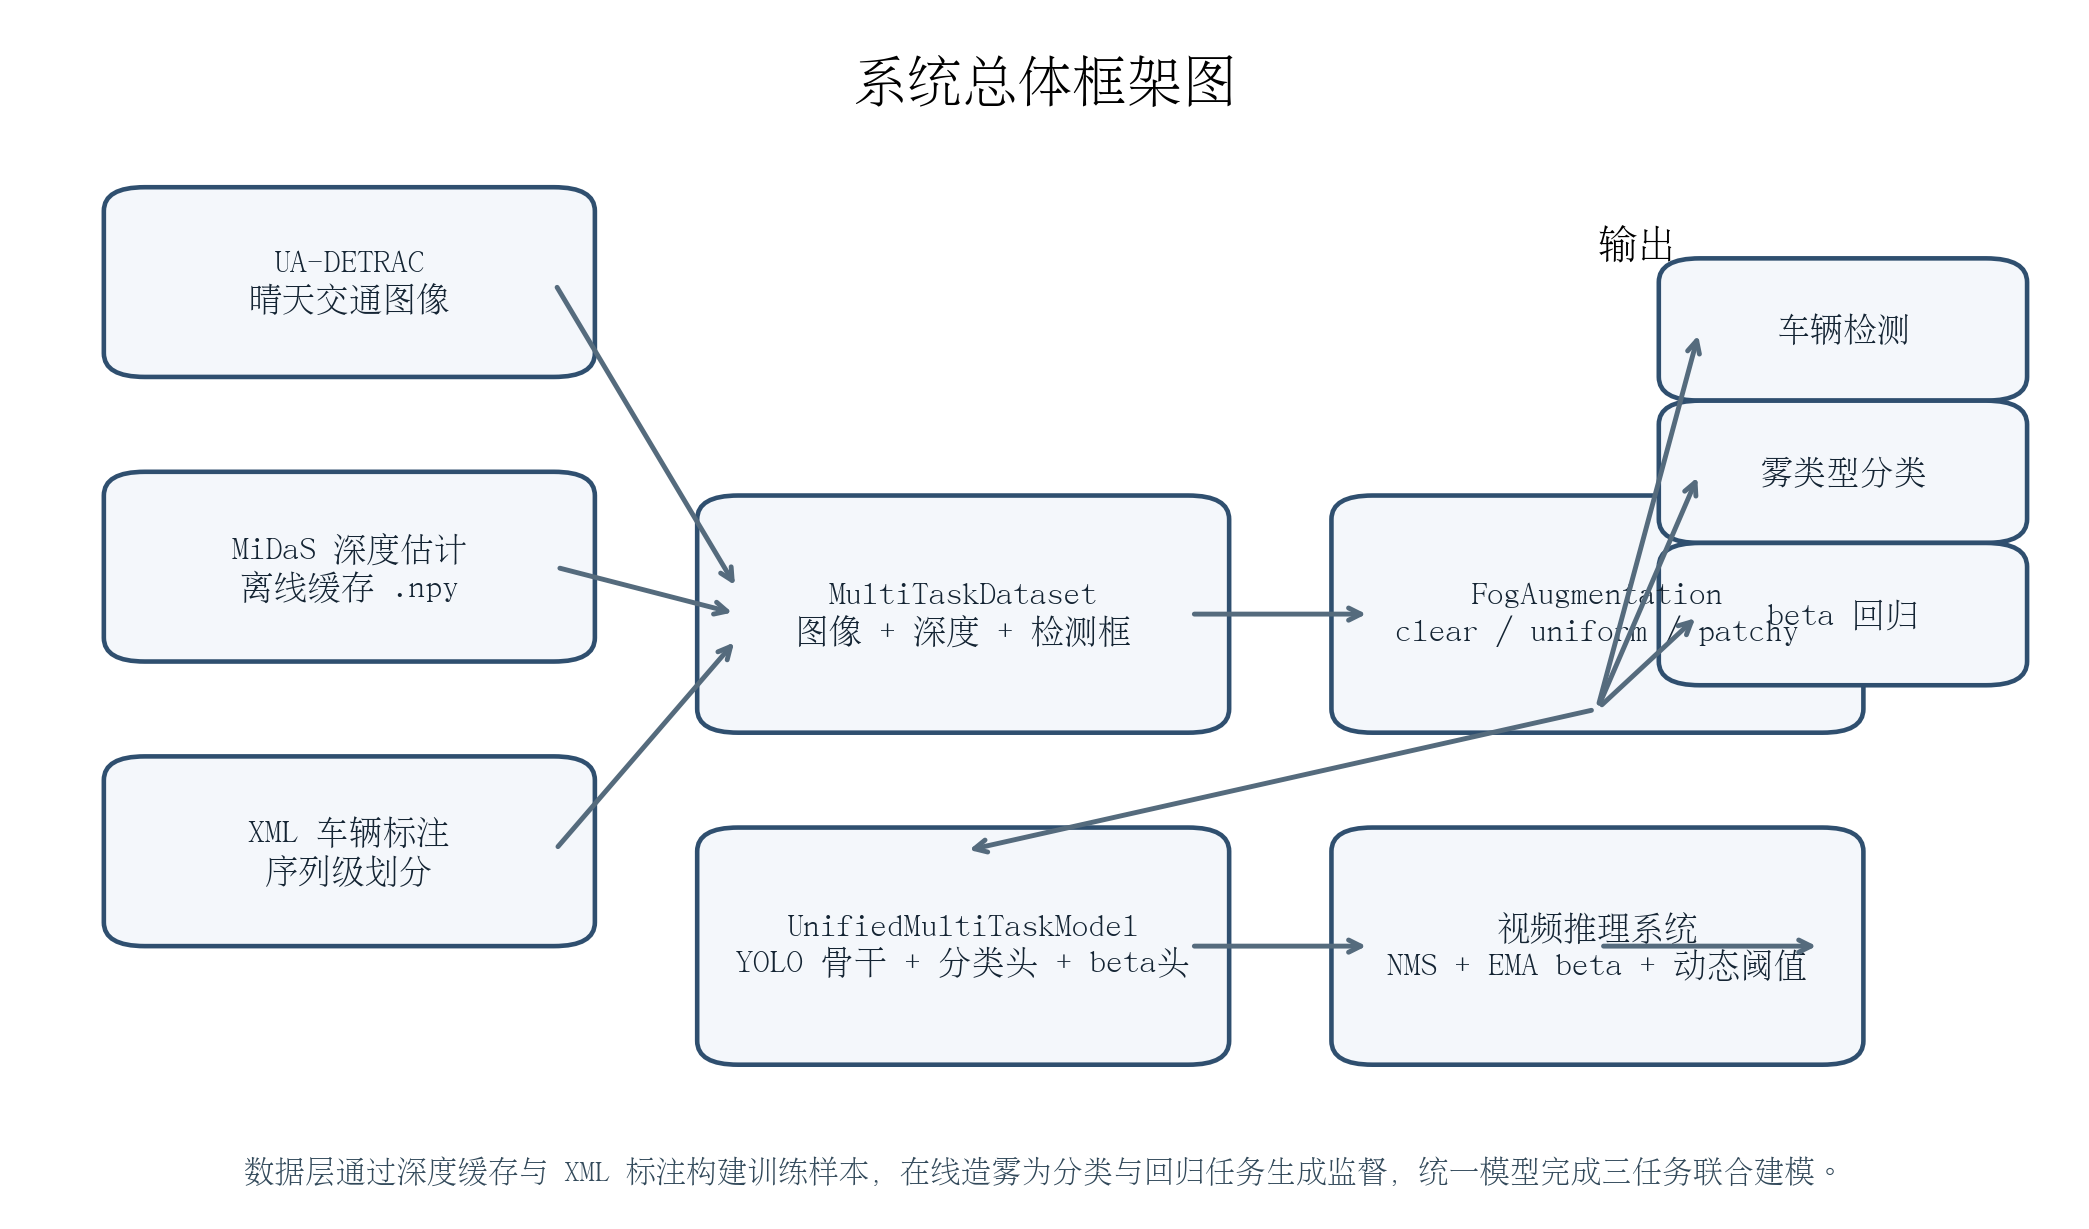
\includegraphics[width=0.95\textwidth]{fig_01_system_overview.png}
  \caption{系统总体框架图}
  \label{fig:system_overview}
\end{figure}

\section{系统模块划分}

从代码实现角度看，本文系统可划分为以下几个核心模块。

\begin{enumerate}[leftmargin=2.5em]
\item 配置模块。位于 \code{src/config.py}，统一管理数据路径、模型参数、训练超参数、物理参数、推理阈值和导出目录，是训练、推理和导出的统一真实配置源。
\item 数据模块。位于 \code{src/data/}。其中 \code{dataset.py} 负责构建多任务训练数据集，\code{depth_estimator.py} 负责深度估计与缓存生成，\code{preparer.py} 则提供离线 YOLO 数据集整理功能。
\item 模型模块。位于 \code{src/model/}。其中 \code{fog_augmentation.py} 负责在线造雾增强，\code{unified_model.py} 负责统一多任务模型结构定义。
\item 训练模块。位于 \code{src/train.py}，负责数据装载、损失计算、联合训练、续训、QAT 和权重保存。
\item 推理模块。位于 \code{src/inference.py}，负责加载统一模型并对视频帧进行推理与可视化。
\item 辅助脚本模块。位于 \code{scripts/}，用于实现数据审计、深度缓存补算、训练前自检、逐行文档生成以及本文后续新增的混合推理脚本等。
\end{enumerate}

\section{系统特点}

本文系统具有以下几个鲜明特点。

其一，真实配置源统一。与许多“文档配置和代码配置并存、易造成版本漂移”的项目不同，本文明确以 \texttt{src/config.py} 作为真实配置入口，使训练、推理和导出均围绕统一参数展开。

其二，训练与推理几何空间保持一致。无论是数据集侧的 letterbox 处理，还是推理时的视频帧预处理，本文均采用一致的几何对齐方式，从而降低训练-推理几何失配带来的性能波动。

其三，系统从一开始就考虑了部署和容错。例如，训练脚本支持缺失深度缓存自动补算；推理系统支持权重自动回退；导出脚本支持 ONNX 输出；量化路径保留了 QAT 与 INT8 转换能力。这使得本项目不仅是一个研究方法，也是一套具备工程闭环特征的原型系统。

其四，系统具有较强的扩展性。后续若要引入真实雾视频监督、加入可见度等级估计、融合更多交通气象传感器数据，均可在当前框架上继续演进，而无需完全推翻已有实现。

\chapter{数据集构建与在线团雾合成方法}

\section{原始数据集选择与分析}

本文选用 UA-DETRAC 作为基础交通视频数据来源。该数据集具有以下优点：第一，数据来自固定道路监控摄像头，与本文研究的高速公路监控场景在视角上更接近；第二，包含连续视频帧和配套 XML 标注，便于开展序列级划分与检测监督构建；第三，车辆目标丰富，适合用作单类 \texttt{vehicle} 检测任务的数据基础。虽然 UA-DETRAC 并不是专门的雾天数据集，但其清晰天气样本丰富、结构规范，因此非常适合作为“清晰交通数据 + 在线造雾”路线中的基底数据。

根据当前工作区运行时统计结果，原始训练数据目录中共包含 60 个监控序列，测试目录中包含 40 个监控序列。按照当前代码中的随机种子、帧步长和序列级划分策略，运行时实际得到训练集 48 个序列、67790 个样本，验证集 12 个序列、16001 个样本。进一步统计可知，当前训练集包含 66811 个有标注样本、473719 个检测框，验证集包含 15274 个有标注样本、124562 个检测框。这些统计来自本文项目在当前环境中的真实运行，而不是静态文档估计值，因此更能反映论文撰写时系统的真实数据基础。

这组数据规模对于毕业设计和工程原型而言已经具备较高的可用性。一方面，车辆目标数量足够支撑单类检测训练；另一方面，固定监控视频序列的数据组织形式，十分适合研究“相同机位、不同气象退化下的联合感知问题”。然而，该数据集也存在局限：它缺少真实团雾标签，无法直接监督雾分类与浓度回归；此外，由于原始标注只覆盖车辆目标，因此天气任务必须通过合成方式构建监督信号。

\begin{figure}[htbp]
  \centering
  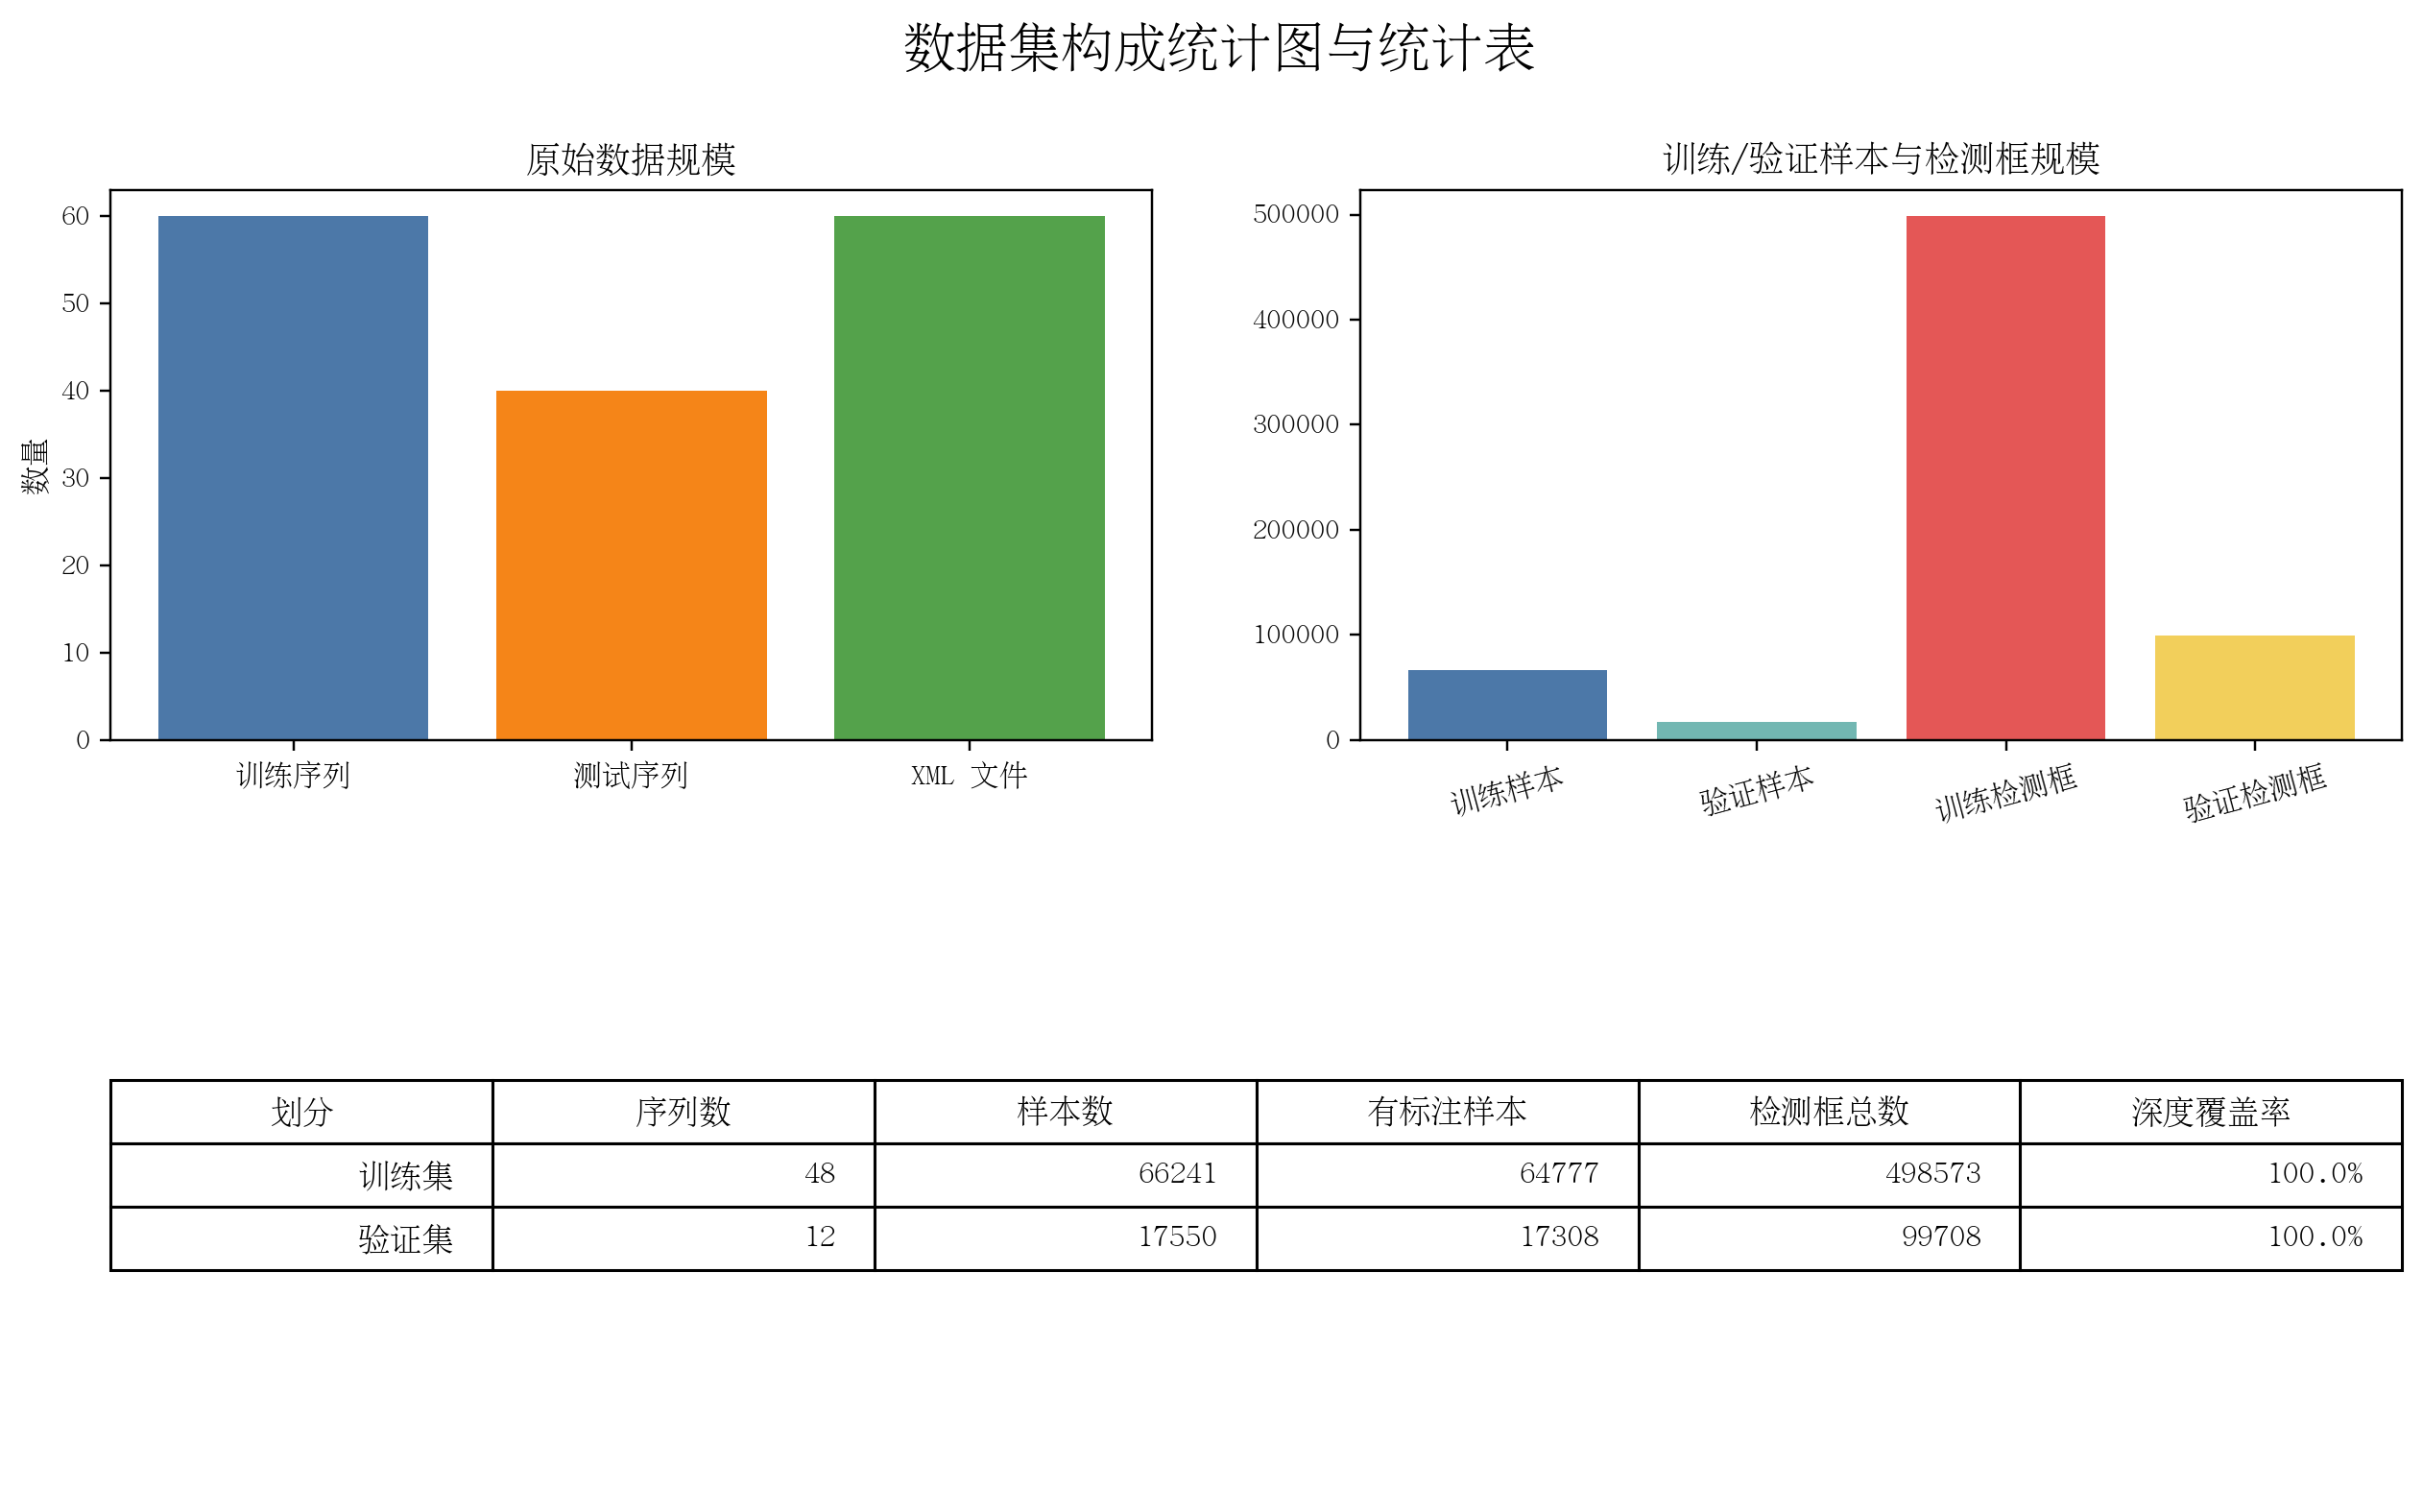
\includegraphics[width=0.95\textwidth]{fig_04_dataset_statistics.png}
  \caption{数据集构成统计图与统计表}
  \label{fig:dataset_statistics}
\end{figure}

\section{序列级训练集与验证集划分}

在交通监控视频场景中，若按图像帧随机划分训练集和验证集，会使同一摄像头、同一时段甚至相邻帧同时出现在训练集和验证集中，从而导致严重的数据泄漏问题。模型可能因为记住了背景结构、车道位置和局部目标外观，而在验证阶段获得虚高结果。因此，本文在 \texttt{src/utils.py} 中实现了按序列名排序、打乱并基于随机种子切分的 \texttt{split\_sequence\_names()} 逻辑，在 \texttt{MultiTaskDataset} 中严格按视频序列划分训练集和验证集。

这种划分方式有两个好处。其一，它保证了训练集与验证集之间不存在相邻帧泄漏，更符合视频任务的真实评估要求。其二，它使深度缓存预计算、数据审计脚本和训练主流程共享同一划分规则，从而避免“训练划分一套，预计算划分另一套”的工程混乱。当前系统中，\texttt{Config.TRAIN\_RATIO = 0.8}，随机种子为 42，因而每次重新构建数据集时都可得到稳定一致的 train/val 拆分结果。

\section{深度缓存预计算与管理}

由于本文在线造雾依赖场景深度信息，而训练集规模较大，若在每个 epoch 中为每一张图重复运行 MiDaS 推理，将显著增加训练时间并带来额外不稳定因素。因此，本文采用“训练前离线预计算 + 训练时直接读取缓存”的方式管理深度图。

具体实现为：首先调用 \texttt{DepthEstimator} 使用 MiDaS\_small 对每张图像估计相对深度，随后将深度图插值回原图尺寸、归一化到 \texttt{[0,1]} 区间，并统一处理为“0 表示近、1 表示远”的深度约定，再以 \texttt{.npy} 格式保存到 \texttt{outputs/Depth\_Cache/}。缓存文件命名规则为 \texttt{序列名\_图像名.npy}，例如某序列中的 \texttt{img00001.jpg} 对应缓存文件 \texttt{MVI\_xxxxx\_img00001.jpg.npy}。这种命名规则使图像、序列和深度缓存之间的映射关系简单直接，便于在 \texttt{\_\_getitem\_\_()} 中快速定位。

从当前运行情况来看，深度缓存覆盖已经完整。工作区中 \texttt{outputs/Depth\_Cache} 的 \texttt{.npy} 文件数量与原始训练图像总量一致，训练前 smoke test 也确认在抽查范围内训练集和验证集未发现缺失缓存。训练脚本还进一步实现了自动补算策略：即使用户没有手动执行深度预计算，只要发现 train/val 任一侧存在缺失缓存，也会在正式训练前自动补齐。这种设计显著增强了系统鲁棒性，降低了“训练半途因缺文件崩溃”的风险。

\section{多任务数据集设计}

本文的多任务数据集定义在 \texttt{src/data/dataset.py} 中，其核心目标并非输出离线雾图，而是为在线造雾和统一模型训练提供完整输入。每个样本返回四类信息：清晰图像张量、对应深度图张量、检测类别张量和检测框张量。其中，图像与深度图用于在线生成雾样本，检测类别与框则用于构造检测监督。

在具体实现中，数据集完成了以下几项关键工作：

\begin{enumerate}[leftmargin=2.5em]
\item 从原始序列目录扫描样本并建立 \code{(img_path, seq, img_name)} 三元组索引；
\item 预加载各序列 XML 标注，建立按 \code{sequence}、\code{frame_num} 与 \code{boxes} 组织的层级映射，提高 \code{__getitem__()} 性能；
\item 在样本读取阶段读取清晰 RGB 图像与对应深度缓存；
\item 将原始绝对坐标框转换为与图像空间对齐的 \codeword{xyxy} 表达，再统一转换为归一化 \codeword{xywh}；
\item 当指定 \code{img_size} 时，对图像和深度图共同执行 letterbox 或缩放处理，并同步变换检测框。
\end{enumerate}

值得强调的是，本文的输入空间处理保持了较强的一致性。无论是训练还是推理，系统都优先使用 letterbox，而不是简单拉伸。这是因为固定监控画面中横纵比往往固定，若直接拉伸至正方形，将改变车辆形状与车道透视比例，影响检测与天气判别的一致性。

\section{在线团雾合成方法}

为在缺乏大规模真实团雾标注数据的前提下训练雾分类与浓度回归任务，本文设计了位于 \texttt{src/model/fog\_augmentation.py} 中的在线造雾模块 \texttt{FogAugmentation}。该模块在 GPU 上实时运行，不预生成离线雾图，从而具有以下优势：一是节省磁盘空间；二是每轮训练都可动态生成不同参数组合，提升样本多样性；三是避免离线数据版本膨胀与管理复杂度。

在线造雾共构造三类天气样本：

\begin{itemize}[leftmargin=2em]
\item \texttt{clear}：无雾样本，保持原图像不变，并将 beta 标签置为 0；
\item \texttt{uniform}：均匀雾样本，整幅图像按统一散射参数退化；
\item \texttt{patchy}：团雾样本，在深度基础上叠加低频噪声，使局部区域雾强度发生变化。
\end{itemize}

在参数采样方面，系统根据 \texttt{Config} 中设置的物理范围对 beta 与大气光 A 进行随机采样，其中 \texttt{BETA\_MIN = 0.02}、\texttt{BETA\_MAX = 0.1}、\texttt{A\_MIN = 0.7}、\texttt{A\_MAX = 0.95}。对于 \texttt{uniform} 样本，系统根据深度图计算透射率，并对极端值进行裁剪，防止图像完全变白或几乎无雾。对于 \texttt{patchy} 样本，则先生成低分辨率随机噪声并双三次上采样到原图大小，再将该噪声作为有效深度调制因子，使浓雾和淡雾能够在同一画面局部并存。

从任务监督角度看，这一模块具有双重作用。首先，它提供雾类别标签，支撑分类头训练；其次，它输出实际用于生成雾图的 beta 值，支撑回归头学习。这意味着雾分类与 beta 回归不再依赖人工标注，而是由在线合成过程自动生成监督信号。虽然这种监督属于“合成标签”，与真实物理能见度并不严格等价，但它为模型学习“相对雾强度”提供了稳定、连续且可控的训练信号。

\section{在线造雾策略的合理性分析}

为何本文不直接收集雾天视频进行监督，而选择清晰数据加在线造雾？原因主要有三点。

首先，真实团雾样本获取成本高且分布稀疏。团雾往往发生在特定路段、特定季节和特定时段，不易形成稳定的大规模数据集。即使采集到视频，如何给每一帧准确赋予可比的浓度标签也是困难问题。

其次，在线造雾虽然不能完全还原真实世界，但能够用统一的物理启发生成可控监督，并通过大规模多样化组合提升模型学习到的退化规律。对于毕业设计与工程原型阶段，这是一种成本与效果之间较为合理的折中。

再次，本文关注的是“监测系统原型”而非高精度气象物理反演器。因此，beta 在本文中首先被视作“与雾强度正相关、可回归、可解释、可平滑”的相对指标，而不是需要绝对匹配气象站能见度的严格物理量。只要该指标能够稳定反映从清晰到严重退化的变化趋势，并能与视频检测和风险显示联动，就具备了实际价值。

\begin{figure}[htbp]
  \centering
  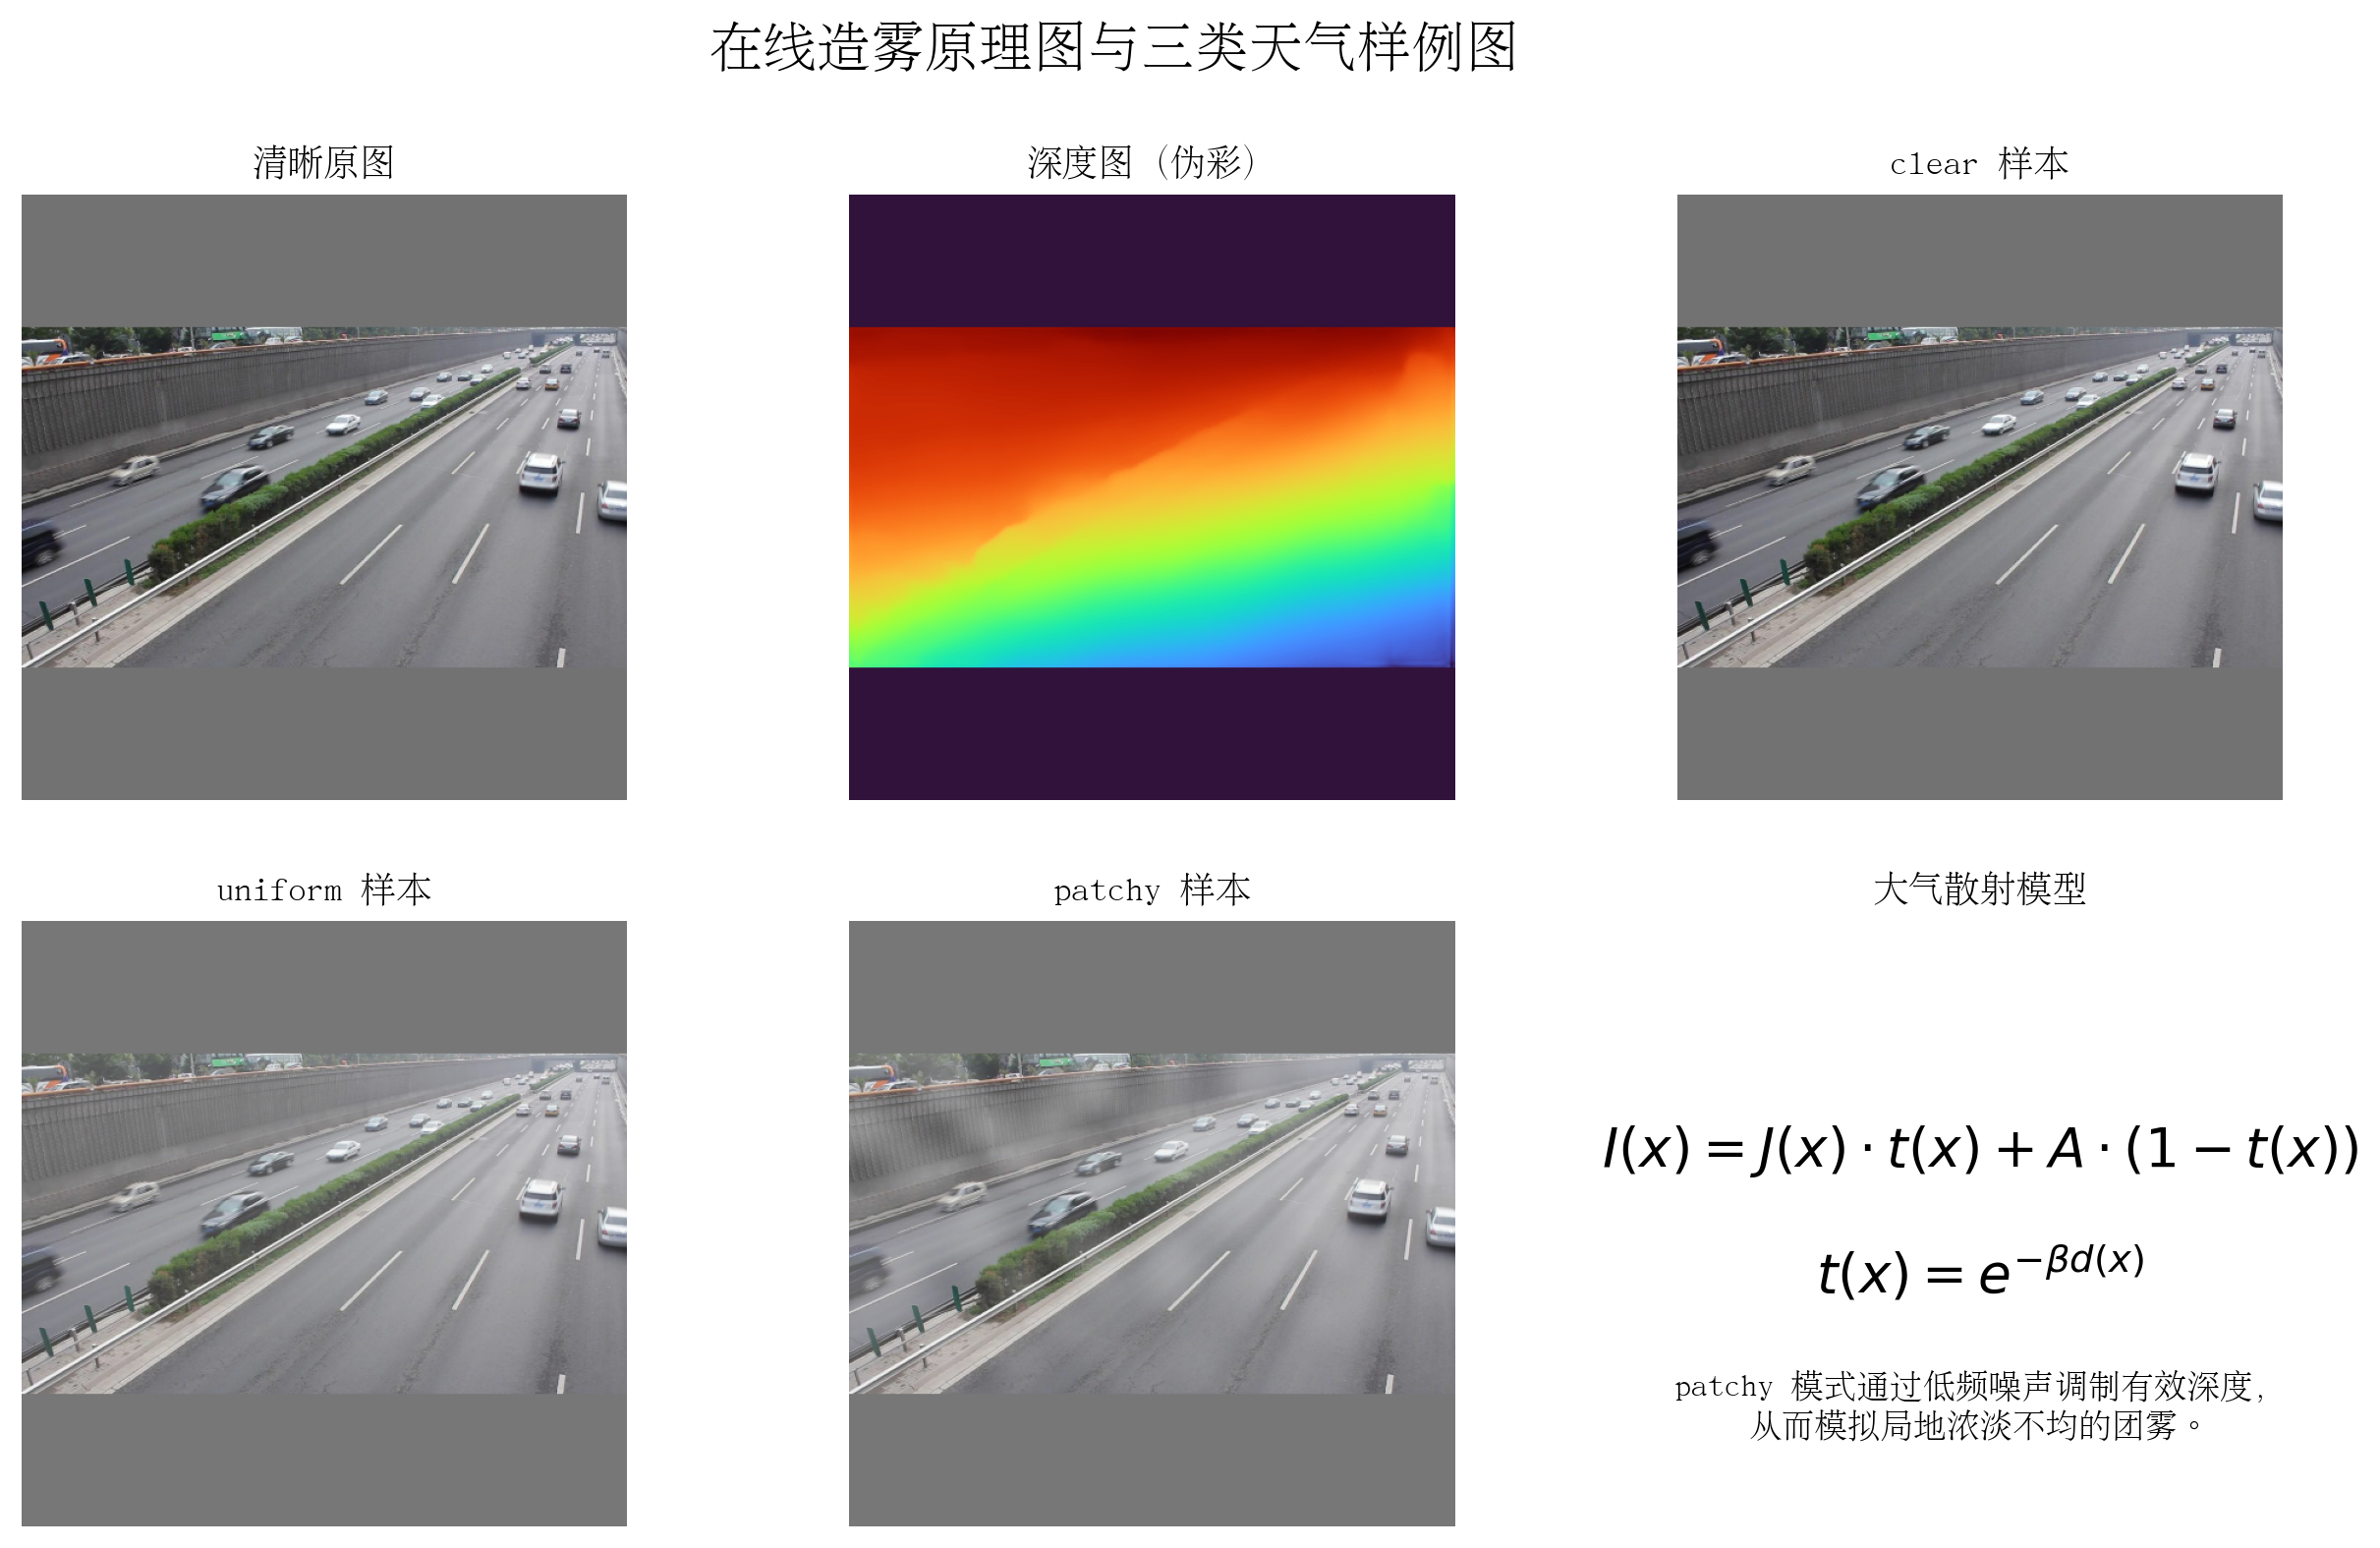
\includegraphics[width=0.95\textwidth]{fig_02_fog_augmentation_examples.png}
  \caption{在线造雾原理图与三类天气样例图}
  \label{fig:fog_augmentation_examples}
\end{figure}

\chapter{统一多任务模型设计与训练优化}

\section{模型总体结构}

本文统一多任务模型定义在 \code{src/model/unified_model.py} 中，命名为 \code{UnifiedMultiTaskModel}。模型整体结构采用“YOLO 共享主干 + 两个附加头”的形式，即：

\begin{enumerate}[leftmargin=2.5em]
\item 使用 YOLO 主干和颈部完成多尺度特征提取；
\item 保留 YOLO 检测头用于车辆检测；
\item 在高层共享特征图上增加雾分类头；
\item 在同一共享特征图上增加 beta 回归头。
\end{enumerate}

这种结构的核心思想是：车辆检测需要局部多尺度感知，而天气识别和雾浓度估计更偏全局语义；因此，将这三项任务放在同一主干上，可以在兼顾速度的同时利用高层共享特征实现协同学习。相比使用三套独立模型，这种设计具有参数更少、推理链路更短、部署更容易的优势。

\begin{figure}[htbp]
  \centering
  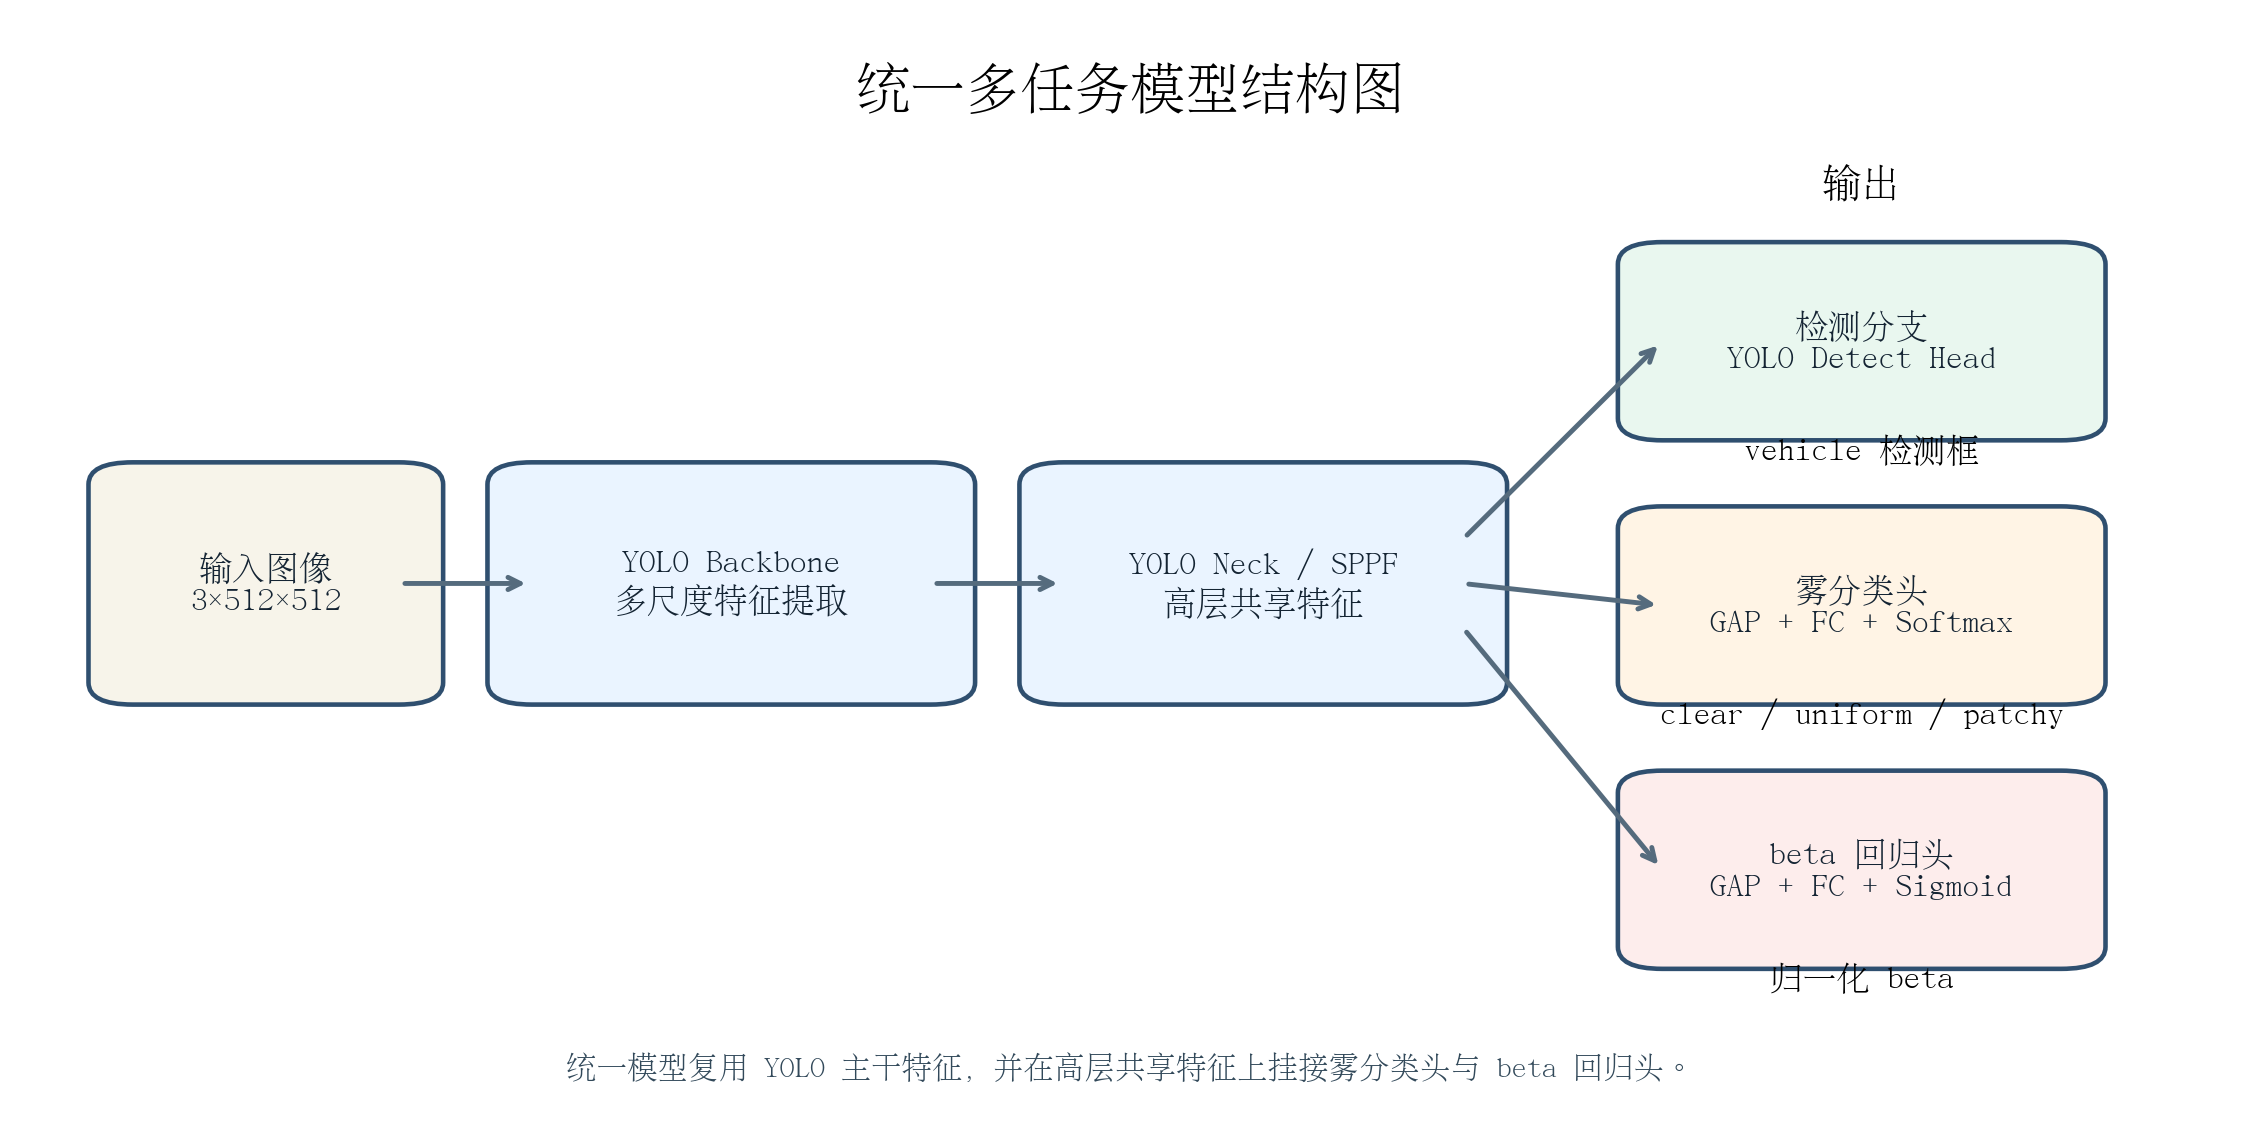
\includegraphics[width=0.92\textwidth]{fig_03_model_structure.png}
  \caption{统一多任务模型结构图}
  \label{fig:model_structure}
\end{figure}

\section{单类车辆检测头适配}

本文场景主要关注道路车辆，而不需要保留通用目标检测中的 80 类全部语义。因此，系统在配置中明确设定 \texttt{NUM\_DET\_CLASSES = 1}，类别名称为 \texttt{["vehicle"]}。然而，基础权重 \texttt{yolo11n.pt} 原本是在多类别数据上训练得到的，其检测头输出维度与单类任务不一致。为解决这一问题，本文在模型初始化阶段检测基础模型最后一层的类别数；若与当前任务不一致，则重建单类 \texttt{DetectionModel}，并从原始权重中选择形状兼容的参数进行非严格加载。

这种适配策略十分关键。若直接以严格模式加载多类权重到单类模型，程序会因 shape 不匹配失败；若完全放弃预训练权重，又会失去 backbone 和 neck 中已学到的大量通用视觉特征。本文采取的折中方案是：保留能复用的主干参数，仅重置类别不兼容的检测头部分。这样既能保留迁移学习优势，又能让模型适配当前道路监控单类检测任务。

\section{雾分类头设计}

雾分类头的输入来自 YOLO 高层共享特征，而非直接使用原图像。其结构为：

\begin{center}
\small
\code{AdaptiveAvgPool2d -> Flatten -> Linear(256)}\\
\code{-> ReLU -> Dropout -> Linear(num_fog_classes)}
\end{center}

之所以采用全局平均池化，是因为雾类型识别更关注整幅画面的整体退化模式，而不是某个局部区域的细节。通过池化操作，模型可将空间特征压缩为全局描述向量，再通过全连接层完成三分类。当前雾类别定义为：

\begin{itemize}[leftmargin=2em]
\item \texttt{clear}
\item \texttt{uniform}
\item \texttt{patchy}
\end{itemize}

这三类设置兼顾了业务可理解性与训练可实现性。\texttt{clear} 表示无雾，\texttt{uniform} 表示均匀低能见度，\texttt{patchy} 则用于表示局地非均匀团雾。在实际管理中，\texttt{patchy} 比 \texttt{uniform} 更值得关注，因为它更容易诱发突发性风险。

\section{beta 回归头设计}

回归头同样基于共享高层特征设计，其结构为：

\texttt{AdaptiveAvgPool2d -> Flatten -> Linear(128) -> ReLU -> Linear(1) -> Sigmoid}

其中最终使用 \texttt{Sigmoid} 将输出压缩到 \texttt{[0,1]} 范围，再在训练与推理阶段按 \texttt{Config.BETA\_MAX} 做缩放。这意味着模型回归的并不是原始物理量纲下的绝对散射系数，而是相对于预设上界的归一化值。当前实现中，回归目标在 clear 样本上被显式置为 0，在有雾样本上由在线造雾过程给出真实采样 beta。因此，该回归头可以被视为学习“当前画面相对于训练雾强度上限的退化程度”。

beta 回归的意义并不只是提供一个数字。对于系统应用而言，连续 beta 值可以进一步用于显示平滑、动态阈值控制、预警等级划分和小地图可视化，因此它是连接模型输出与业务联动的重要桥梁。

\section{多任务前向传播与共享特征提取}

与许多简单封装直接调用 \code{self.yolo(x)} 的方式不同，本文在 \code{forward()} 中手动遍历 \code{self.yolo.model} 各层前向传播，并尝试捕获 SPPF 或检测头前最后一张高层 4D 特征图作为共享特征。这一实现看似复杂，但非常必要。因为若只调用高层封装接口，往往难以在推理结构变化和训练/验证模式差异下稳定获得可供附加头使用的高层特征。

本文采用的共享特征提取策略是：优先捕获 \texttt{SPPF} 层输出；若当前 YOLO 架构中无法明确识别 \texttt{SPPF}，则退化为检测头前最后一张 4D 特征图。这种设计提升了模型对不同 YOLO 规模和结构变体的适应性，也避免了把通道数写死在代码里。

\section{损失函数与联合优化}

训练阶段，检测、分类和回归三项任务同时纳入优化目标。具体而言：

\begin{itemize}[leftmargin=2em]
\item 检测损失直接调用 Ultralytics 提供的 detection loss；
\item 雾分类损失使用 \texttt{CrossEntropyLoss}；
\item beta 回归损失使用 \texttt{MSELoss}。
\end{itemize}

总损失写为：

\[
L = L_{det} + L_{cls} + L_{reg}
\]

虽然当前实现中三项任务权重均为 1.0，但这并不意味着三项损失在数值尺度上天然相等。实际训练中，检测损失往往明显高于雾分类与回归损失，这也是当前日志中“det 占主导，fog\_cls 与 fog\_reg 数值更小”的原因。对此，本文采取两种应对方式：一是通过共享高层特征让天气任务充分利用检测主干已有的表达能力，减轻天气头从零学习的压力；二是在实验设计中预留损失权重调整空间，以便后续根据收敛曲线进一步平衡不同任务。

\section{训练稳定性与工程保护机制}

相比只关注最终精度的论文实现，本文训练脚本在工程稳定性方面做了较多保护设计。

首先，训练过程支持自动续训。系统会在 checkpoint 目录中查找最新权重，若存在则恢复模型、优化器、调度器和 AMP scaler 状态，并从下一个 epoch 继续训练。这对于长时间训练、多次中断和实验迭代都十分重要。

其次，训练过程支持缺失深度缓存自动补算。训练开始前会统计训练集和验证集各自缺少多少深度文件，若有缺失则自动调用预计算流程补齐，避免训练到验证阶段才因文件缺失报错。

再次，脚本支持 AMP 混合精度训练，并监控非有限梯度比例。当前代码中实现了对 \texttt{NaN/Inf} 梯度的检测、告警、阈值判定以及必要时自动关闭 AMP 的恢复策略。这种设计在大 batch、长时间训练或量化感知训练切换中尤为重要。

最后，系统保留了 QAT 与 INT8 转换路径。虽然当前毕业设计阶段更关注功能打通与方法验证，但在 \texttt{src/train.py} 中已经实现了 QAT 准备、observer 修复和 INT8 模型转换流程，为后续边缘部署提供了明确方向。

\section{当前训练状态与续训策略}

在本文撰写时，项目工作区中已经存在一版训练权重和 checkpoint。现有 checkpoint 对应的训练记录显示，系统此前至少完成了首个 epoch 的训练，并保存了 \code{unified_model.pt}、\code{unified_model_best.pt} 以及 \code{checkpoint_epoch_0001.pt}。从工程验证看，这意味着统一模型主链已经能够完成参数更新、权重保存和推理调用；从效果层面看，早期权重在真实下载雾视频上的雾估计已可输出数值，但车辆检测稳定性仍不如直接使用预训练 YOLO11n 的结果，因此本文在系统演示阶段补充实现了混合推理策略。

为了进一步提升雾分类和 beta 回归可靠性，当前系统已在后台执行一轮“短程快速微调”：继续沿用现有 checkpoint，但对每个 epoch 的最大训练 batch 数和验证 batch 数做限制，从而在可接受时间内获得更新权重。这一策略的意义不在于替代完整训练，而在于为论文初稿撰写阶段提供更接近最终状态的参数版本，并为后续实验章节补充完整指标争取时间。

\chapter{视频推理系统设计、可视化与部署实现}

\section{统一模型推理流程}

统一模型推理由 \code{src/inference.py} 中的 \code{HighwayFogSystem} 封装完成。系统首先根据配置自动解析模型权重路径，优先选择 \code{unified_model_best.pt}；若不存在，则回退至 \code{unified_model.pt} 或最新 checkpoint。随后，系统对视频帧执行如下流程：

\begin{enumerate}[leftmargin=2.5em]
\item 读取 OpenCV BGR 帧并转换为 RGB；
\item 按训练阶段一致的规则执行 letterbox 预处理；
\item 输入统一多任务模型，得到检测输出、雾分类 logits 和 beta 回归值；
\item 对检测结果执行 NMS；
\item 对 beta 进行 EMA 平滑；
\item 根据平滑后的 beta 计算自适应置信度阈值；
\item 绘制车辆检测框、雾状态和 beta 信息。
\end{enumerate}

这种推理链保留了训练-推理一致性，也使雾估计不再只是附加文本输出，而是直接参与检测显示策略控制。

\section{动态阈值机制}

在低能见度场景下，固定检测阈值容易造成漏检。若仍使用与晴天相同的较高阈值，模型可能在轻度或中度雾中丢失一些本就较弱的车辆响应。为此，本文在推理阶段设置基础阈值 \code{BASE_CONF_THRES = 0.25}，再根据平滑后的 beta 值进行动态调整。当前代码中的核心思想可以概括为：

\[
conf_{adaptive} = \max(conf_{min}, conf_{base} - k\hat{\beta})
\]

其中 \texttt{conf\_min = 0.15}，\texttt{k = 1.2}。这意味着当雾浓度上升时，系统会适当降低显示阈值，保留更多潜在目标。虽然这种策略还不是严格意义上的风险最优控制，但它体现了一种重要思想：天气感知结果应当反馈到目标检测显示策略，而不是与检测分离。

\section{运行时多流与异步组织}

若运行设备为 CUDA，\texttt{HighwayFogSystem} 会创建预处理流、推理流和后处理流，尽量让不同阶段形成轻量级流水线。虽然在当前项目规模下，多流并不能使每一步都完全并行，但它有助于降低 CPU/GPU 空转等待，使视频演示更加流畅。该设计说明本文在实现中不仅考虑了算法正确性，也兼顾了运行效率与展示效果。

\section{混合推理方案}

在本文工程推进过程中发现：当前统一模型早期训练权重已经能够给出合理的雾分类概率和 beta 数值，但对真实下载雾视频中的车辆检测效果不如原始预训练 \texttt{yolo11n.pt} 稳定。考虑到毕业设计需要尽快形成“车辆 + 雾状态 + 雾浓度”同时可视化的结果，本文进一步实现了位于 \texttt{scripts/hybrid\_fog\_vehicle\_infer.py} 的混合推理脚本。

该脚本采用如下策略：

\begin{itemize}[leftmargin=2em]
\item 用 \texttt{yolo11n.pt} 负责真实视频中的车辆检测；
\item 用统一多任务模型负责雾分类和 beta 估计；
\item 将两者结果在同一视频中叠加显示；
\item 在右下角构建“雾浓度分布图”小地图，用于增强对空间非均匀雾的直观解释。
\end{itemize}

从严格学术角度看，混合推理不等于统一模型最终目标；但从工程验证角度看，它很好地解决了“系统需要立刻可用，而统一模型尚在持续优化中”的现实问题。其意义在于保证整个毕业设计在方法研究与系统演示之间形成平衡。

\begin{figure}[htbp]
  \centering
  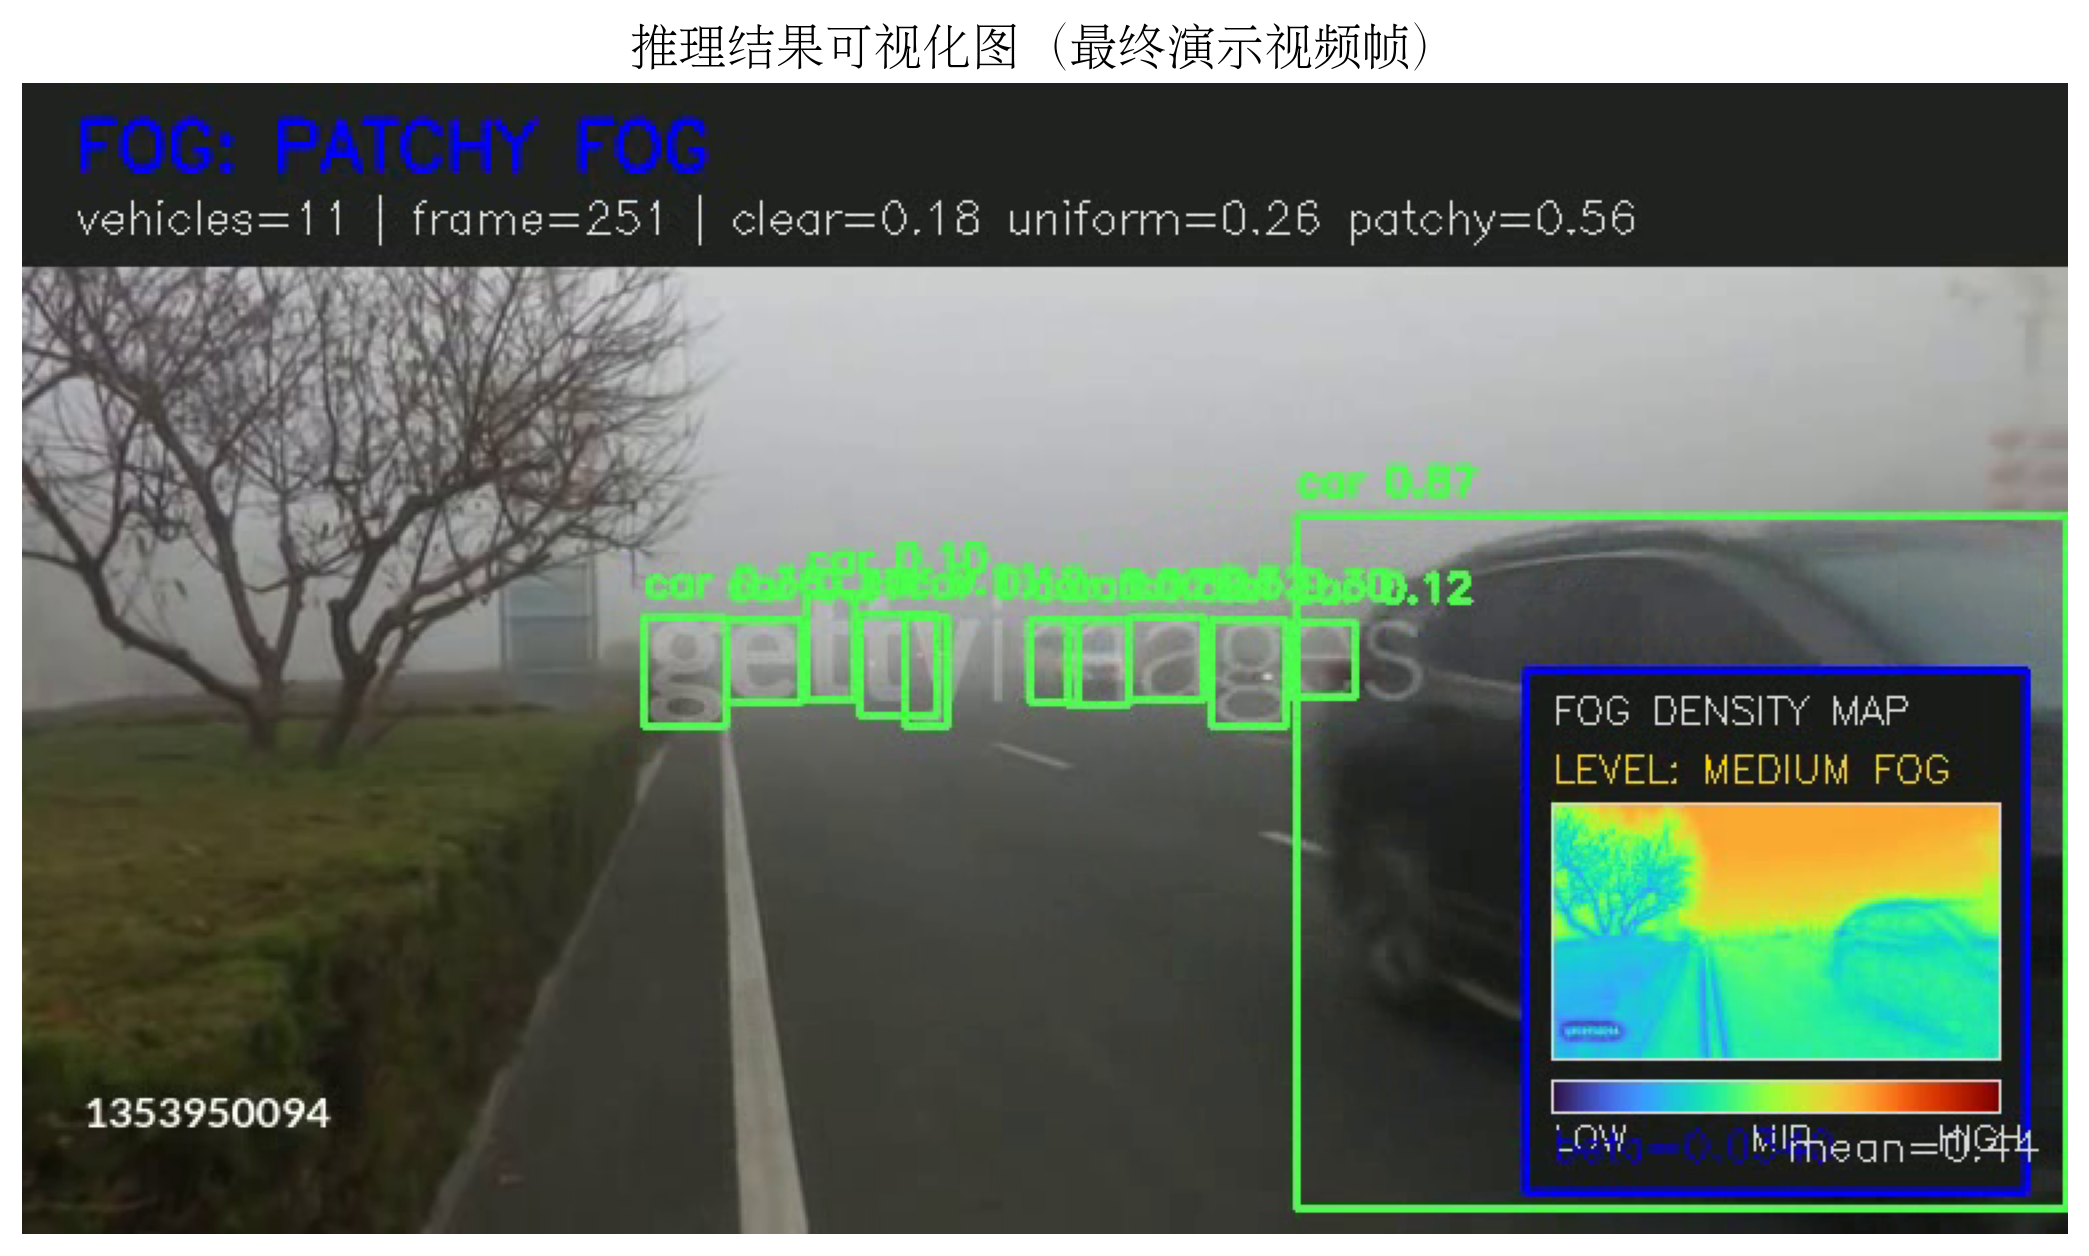
\includegraphics[width=0.94\textwidth]{fig_08_inference_visualization.png}
  \caption{推理结果可视化图}
  \label{fig:inference_visualization}
\end{figure}

\section{雾浓度分布图的构建思路}

需要指出的是，当前统一模型输出的是整帧一个 beta 值，而不是逐像素的雾浓度图。因此，右下角的小地图并不是模型直接回归得到的“真值级空间雾图”，而是一种基于图像局部对比度、饱和度和亮度白化程度估算得到的相对空间雾浓度分布图，并使用全局 beta 对其进行强度校正。

这一设计虽然不是严格物理反演，但具备三个优点：第一，能够在演示视频中直观体现“同一画面不同位置雾强度可能不同”；第二，结合全局 beta 可获得相对稳定的整体浓淡变化；第三，工程实现简单，不需要额外训练密集预测网络。对于论文初稿和系统展示阶段，这种设计已经具有较强的解释性。

\begin{figure}[htbp]
  \centering
  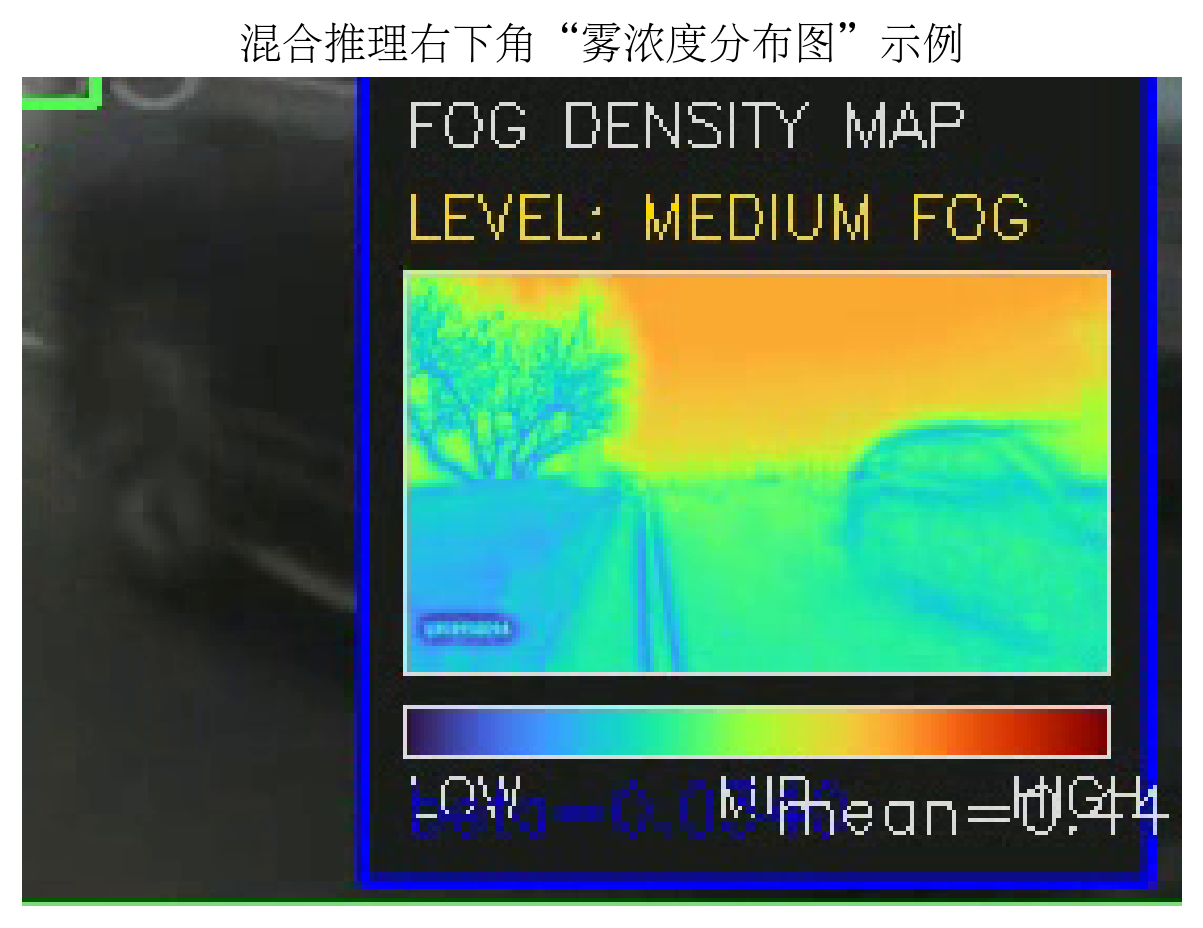
\includegraphics[width=0.65\textwidth]{fig_09_fog_map_example.png}
  \caption{混合推理右下角雾浓度分布图示例}
  \label{fig:fog_map_example}
\end{figure}

\section{导出与部署路径}

为了使本文方法具备更明确的工程延展性，项目还实现了 \texttt{src/export.py} 导出脚本。该脚本可将统一模型导出为 ONNX，并给出 TensorRT INT8 引擎构建示例和 Jetson 部署提示。训练脚本中则保留了 QAT 和 INT8 转换路径。虽然本文目前仍以桌面 GPU 环境下的模型训练和视频推理为主，但从代码结构上看，后续迁移到边缘设备、收费站终端或路侧计算节点具备可操作基础。

\chapter{实验结果与分析}

\section{引言}

在完成系统总体设计、数据构建、模型训练以及推理部署实现之后，论文需要进一步回答两个问题：第一，当前方法在训练和验证层面取得了怎样的定量结果；第二，当前工作区中的不同权重分支、不同推理路线以及误检治理链在工程上究竟表现如何。本章将结合正式训练摘要、正式基准评估、UA-DETRAC 标准检测指标、典型误差案例和静止误检治理产物，对本文系统的实验结果进行集中分析。

\section{实验目的}

本文实验并非只为了给出某一个孤立精度数值，而是围绕以下五个目标展开：

\begin{enumerate}[leftmargin=2.5em]
\item 验证“深度缓存 + 在线造雾 + 统一多任务模型”主链路在当前工程环境中能够稳定运行；
\item 验证统一模型能否同时输出车辆检测、雾类型分类和 beta 回归结果，并形成可解释的视频级表现；
\item 通过正式训练与基准评估判断当前哪一版权重最适合作为论文正式参考点；
\item 评估统一路线与混合路线在真实雾视频和晴天对照视频片段上的差异，明确当前系统真正的短板；
\item 验证静止假车误检治理链是否已经从“概念想法”发展为可记录、可复核、可回灌的工程闭环。
\end{enumerate}

因此，本文实验评价体系不再局限于单一训练损失或单个视频截图，而是同时覆盖训练曲线、离线路线评估、多模型基准评估、候选模型门槛判定结果以及静止误检治理产物。

\section{实验环境}

实验运行环境如下：

\begin{itemize}[leftmargin=2em]
\item Python 3.13.12
\item PyTorch 2.12.0.dev20260406 + CUDA 13.0
\item torchvision 0.27.0.dev20260406
\item Ultralytics 8.4.34
\item NumPy 2.4.3
\item GPU：NVIDIA GeForce RTX 5070 Ti Laptop GPU，显存约 12 GB
\end{itemize}

其中，深度学习训练与推理框架分别基于 PyTorch 与 Ultralytics 的官方实现组织\cite{pytorchDocs,ultralyticsDocs}。

统一模型与推理系统的关键运行参数包括：

\begin{itemize}[leftmargin=2em]
\item 基础检测权重：\code{yolo11n.pt}
\item 默认检测类别数：1（\code{vehicle}）
\item 雾分类类别数：3（\code{clear / uniform / patchy}）
\item 输入尺寸：512
\item beta 范围：0.02 \textasciitilde{} 0.10
\item 推理基础阈值：0.25
\item beta 平滑与阈值联动：EMA + adaptive confidence
\end{itemize}

从工程角度看，这样的配置具有两个优点：其一，能够在 12GB 级别显存设备上完成训练、验证与视频推理；其二，QAT、ONNX 与 TensorRT 路径均已保留，后续向更轻量设备迁移时不必重写主流程。

\section[数据统计与 benchmark\textunderscore{}v1]{数据统计与 benchmark\textunderscore{}v1}

\subsection{训练数据}

基于当前工作区的真实运行结果，训练与验证数据规模如表~\ref{tab:dataset_split_stats} 所示。

\begin{table}[htbp]
  \centering
  \caption{训练集与验证集规模统计}
  \label{tab:dataset_split_stats}
  \small
  \begin{tabular}{@{}lrrrr@{}}
    \toprule
    划分 & 序列数 & 样本数 & 有标注样本数 & 检测框总数 \\
    \midrule
    训练集 & 48 & 67790 & 66811 & 473719 \\
    验证集 & 12 & 16001 & 15274 & 124562 \\
    \bottomrule
  \end{tabular}
\end{table}

与此同时，当前原始训练数据目录共包含 60 个监控序列，测试目录包含 40 个序列；深度缓存文件数量已经与原始训练图像数量对齐，说明 \code{outputs/Depth_Cache} 中的 \code{.npy} 文件覆盖完整。对本文而言，这一点非常重要，因为它意味着论文中的训练结论不是建立在“少量手工挑样本”的临时环境上，而是建立在已经整理完毕的真实数据工作区上。

\subsection{视频资产}

为避免“不同模型用不同视频、不同采样策略比较”的混乱情况，本文冻结了一版 \code{benchmark_v1} 视频集。该视频集由 1 段真实雾视频和 4 段由 UA-DETRAC 构造的晴天对照视频片段组成\cite{uadetrac}。按照本轮正式基准评估的采样设置，其构成如表~\ref{tab:benchmark_v1_assets} 所示。

\begin{table}[htbp]
  \centering
  \caption{\code{benchmark_v1} 视频集构成}
  \label{tab:benchmark_v1_assets}
  \small
  \begin{tabular}{@{}p{3.0cm}p{2.2cm}p{4.9cm}r@{}}
    \toprule
    视频标签 & 场景类型 & 来源说明 & 抽样帧数 \\
    \midrule
    Getty 雾视频 & 真实雾视频 & 根目录真实雾天监控视频 & 168 \\
    稀疏车流对照 & 晴天稀疏车流对照 & UA-DETRAC 序列 \code{MVI_40152} & 60 \\
    中等车流对照 & 晴天中等车流对照 & UA-DETRAC 序列 \code{MVI_20033} & 60 \\
    较重车流对照 & 晴天较重车流对照 & UA-DETRAC 序列 \code{MVI_20011} & 60 \\
    密集车流对照 & 晴天密集车流对照 & UA-DETRAC 序列 \code{MVI_20035} & 60 \\
    \midrule
    合计 & -- & 1 段真实雾视频 + 4 段晴天对照视频 & 408 \\
    \bottomrule
  \end{tabular}
\end{table}

与只使用单段真实雾视频相比，引入多段晴天对照视频片段的意义在于：它把统一模型的主要短板暴露得更加明确。若一个权重只能在单段雾视频上表现尚可，却在多段晴天交通对照视频上持续丢失检测能力，那么该权重并不适合作为最终工程路线的检测主模型。

\section{评价指标}

当前项目的评价指标分为两层。

\subsection{训练指标}

第一层是训练过程中的学习指标，包括：

\begin{itemize}[leftmargin=2em]
\item 检测损失；
\item 雾分类损失；
\item beta 回归损失；
\item 总训练损失与总验证损失；
\item 是否出现 non-finite gradient；
\item 是否触发 AMP recovery。
\end{itemize}

这些指标主要服务于训练稳定性判断，回答“模型是否在收敛”“是否数值稳定”“某种损失权重策略是否可训练”等问题。

\subsection{视频级指标}

第二层是离线路线评估中的视频级工程指标。与常见目标检测论文不同，当前阶段的真实雾视频并不具备逐框人工标注，因此本文不强行给出缺少标注支撑的 mAP，而是使用更贴近当前业务目标的指标：

\begin{itemize}[leftmargin=2em]
\item \code{mean_count_per_frame}：平均每帧检测数；
\item \code{frames_with_detections_ratio}：非零检测帧占比；
\item \code{weighted_beta_mean}：beta 全局均值；
\item \code{weighted_dominant_switch_rate}：主导雾类别切换率；
\item \code{weighted_beta_abs_delta_mean}：beta 帧间抖动强度；
\item \code{heuristic_persistent_static_fp_per_min}：启发式持续静止误检频率；
\item \code{mean_confirmation_latency_frames}：目标从首次出现到被确认显示的平均延迟；
\item \code{route recommendation}：在统一路线与混合路线之间的综合推荐结果。
\end{itemize}

这些指标与当前代码实现严格对应，尤其对应 \code{scripts/evaluate_inference_routes.py}、\code{scripts/run_multi_model_benchmark.py} 和 \code{scripts/benchmark_candidate_model.py} 中的结构化输出。因此，论文中的实验结论与工作区中的 JSON / CSV 结果之间具有一一对应关系。

在本文定稿阶段，项目进一步补充实现了 \code{scripts/evaluate_uadetrac_detection_metrics.py}，用于在 UA-DETRAC 验证集上统计单类车辆检测的 Precision、Recall、mAP@0.5 和 mAP@0.5:0.95\cite{uadetrac}。因此，当前论文已经同时具备“标准检测指标”和“视频级工程指标”两套评价层次：前者更适合回答清晰天气域上的检测质量问题，后者更适合回答真实视频演示路线该如何选择的问题。

\section[fogfocus\textunderscore{}full 训练结果]{fogfocus\textunderscore{}full 训练结果}

当前论文正式采用的主训练结果来自 \code{outputs/Fog_Detection_Project_fogfocus_full}。这轮训练从 \code{fogfocus} 路线已有 checkpoint 继续，核心意图是：在关闭检测损失、冻结检测器的条件下，更集中地优化雾分类头与 beta 回归头。

本轮训练的关键设置如表~\ref{tab:fogfocus_full_setup} 所示。

\begin{table}[htbp]
  \centering
  \caption{\code{fogfocus_full} 正式训练的关键设置}
  \label{tab:fogfocus_full_setup}
  \small
  \begin{tabular}{@{}p{3.8cm}p{8.2cm}@{}}
    \toprule
    项目 & 取值 \\
    \midrule
    起始 checkpoint & \code{outputs/Fog_Detection_Project_fogfocus/checkpoints/checkpoint_epoch_0004.pt} \\
    输出目录 & \code{outputs/Fog_Detection_Project_fogfocus_full} \\
    总 epoch 数 & 12 \\
    学习率 & $1\times10^{-5}$ \\
    \code{FREEZE_YOLO_FOR_FOG} & 1 \\
    \code{DET_LOSS_WEIGHT} & 0.0 \\
    \code{FOG_CLS_LOSS_WEIGHT} & 1.75 \\
    \code{FOG_REG_LOSS_WEIGHT} & 1.35 \\
    \code{MAX_TRAIN_BATCHES / MAX_VAL_BATCHES} & 0 / 0（不做冒烟测试限制） \\
    \code{SKIP_QAT} & 1 \\
    \bottomrule
  \end{tabular}
\end{table}

训练结果摘要如表~\ref{tab:fogfocus_full_result} 所示。

\begin{table}[htbp]
  \centering
  \caption{\code{fogfocus_full} 正式训练结果摘要}
  \label{tab:fogfocus_full_result}
  \small
  \begin{tabular}{@{}lr@{}}
    \toprule
    指标 & 数值 \\
    \midrule
    最佳验证损失 & 1.0072 \\
    第 12 个 epoch 训练总损失 & 0.9346 \\
    第 12 个 epoch 验证总损失 & 1.0072 \\
    训练阶段 fog classification loss & 0.5340 \\
    验证阶段 fog classification loss & 0.5754 \\
    训练阶段 fog regression loss & $1.322\times10^{-4}$ \\
    是否出现 non-finite gradient & 否 \\
    是否触发 AMP recovery & 否 \\
    \bottomrule
  \end{tabular}
\end{table}

该结果表明，当前系统已经不再停留在“仅能完成一次冒烟测试级试跑”的阶段，而是能够在完整 epoch 条件下稳定推进雾任务优化。尤其是 \code{best_loss = 1.0072} 的出现，使 \code{outputs/Fog_Detection_Project_fogfocus_full/unified_model_best.pt} 成为当前最适合写入论文正式实验部分的雾权重参考点。

\begin{figure}[htbp]
  \centering
  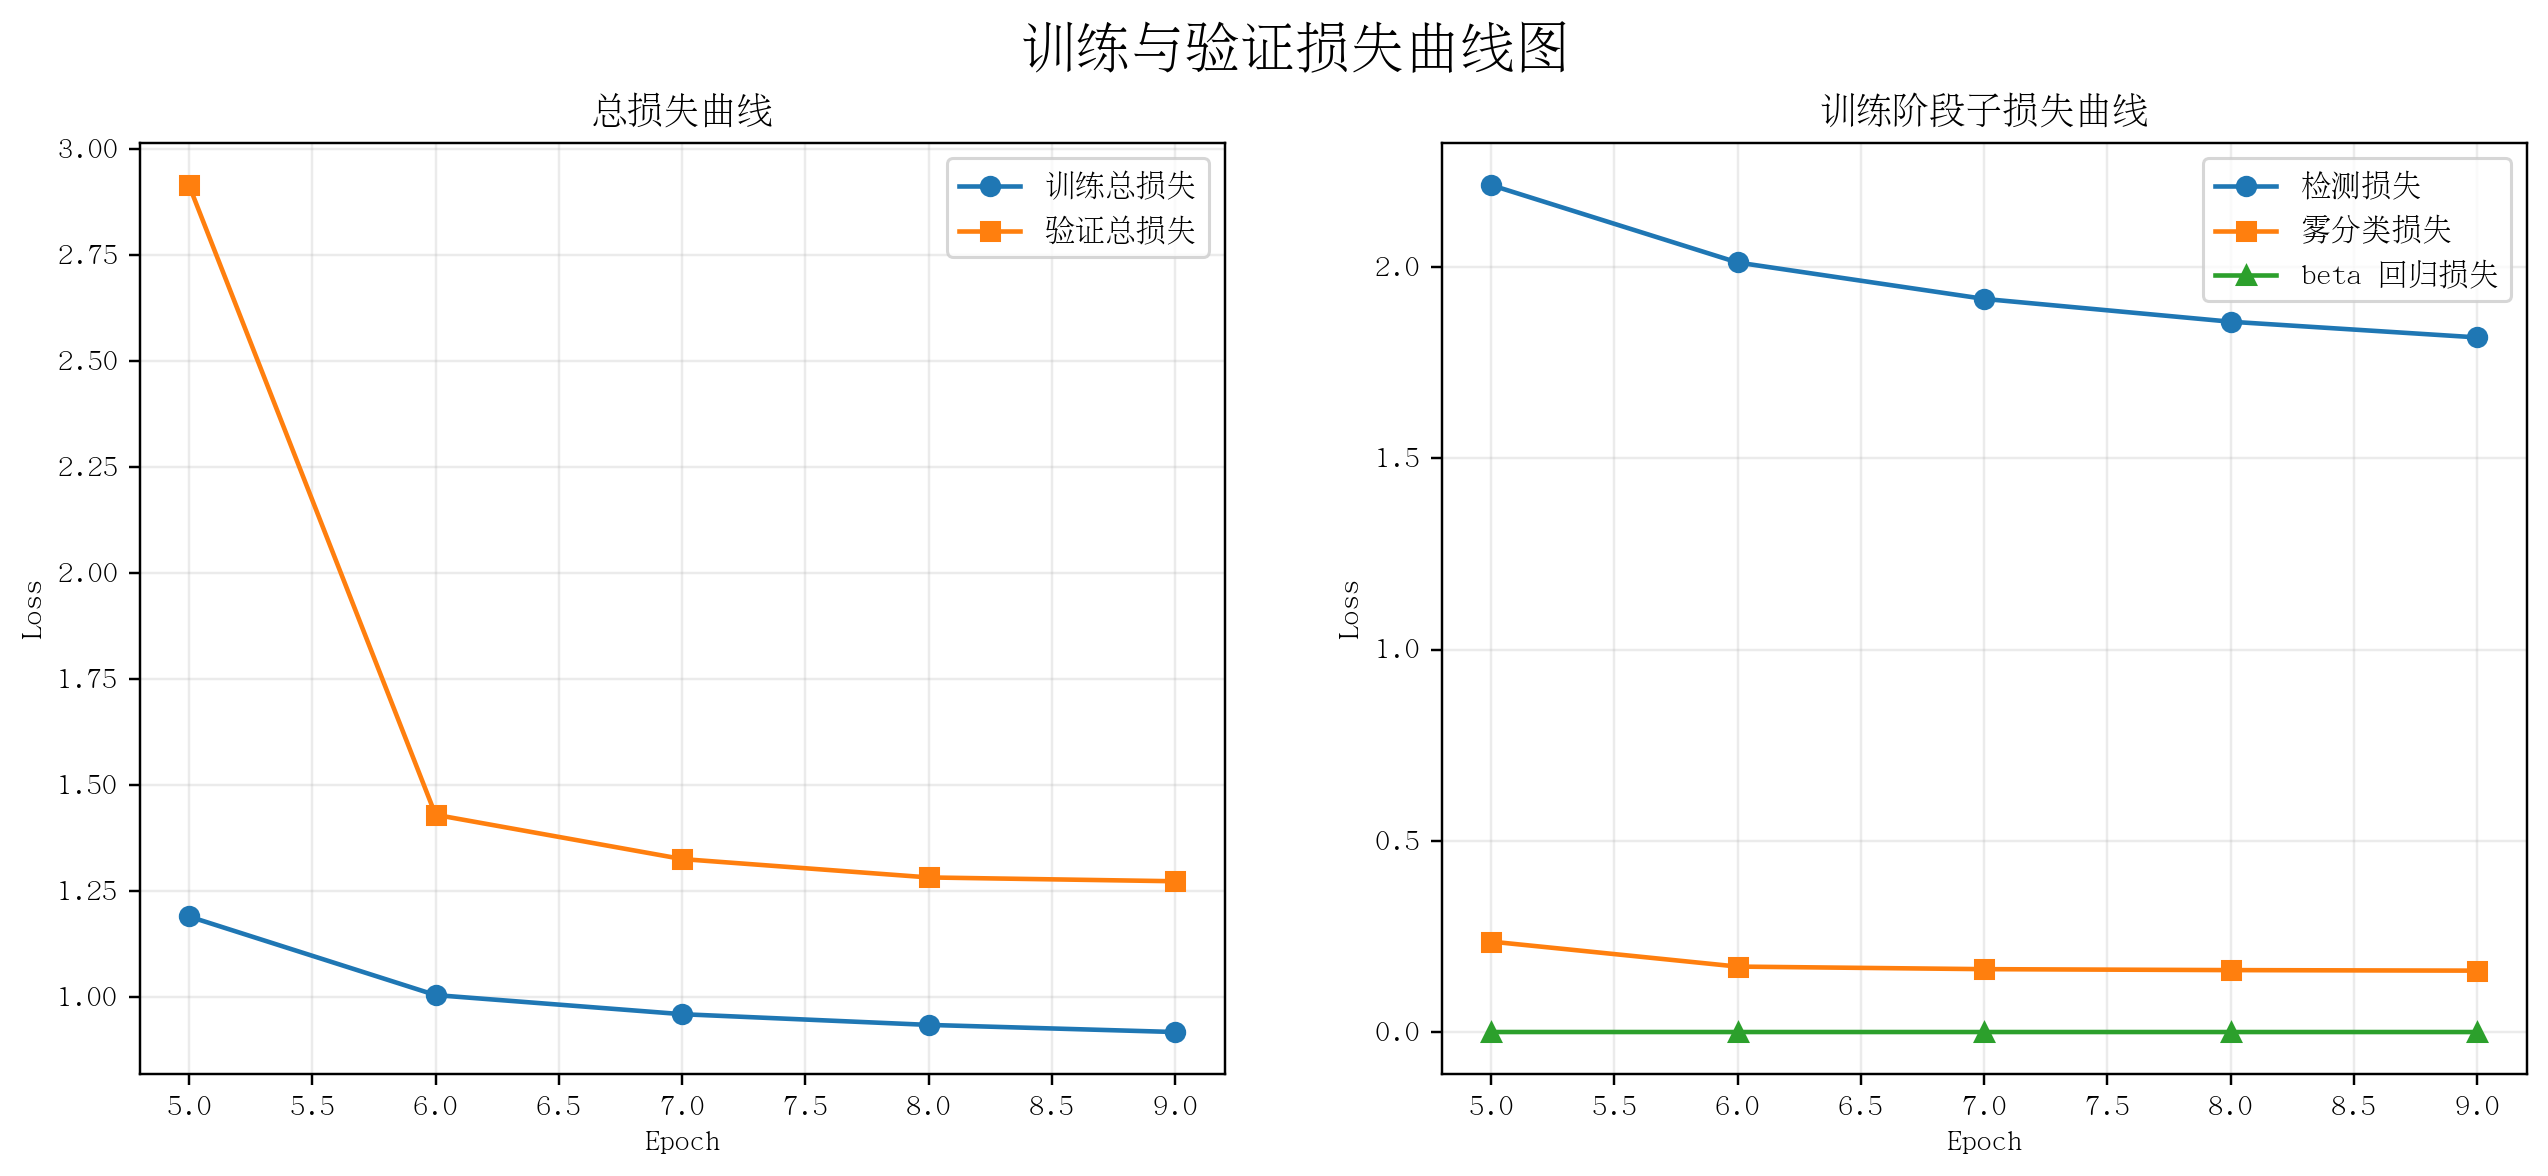
\includegraphics[width=0.96\textwidth]{fig_05_training_validation_loss.png}
  \caption{训练与验证损失曲线图}
  \label{fig:training_validation_loss}
\end{figure}

\begin{figure}[htbp]
  \centering
  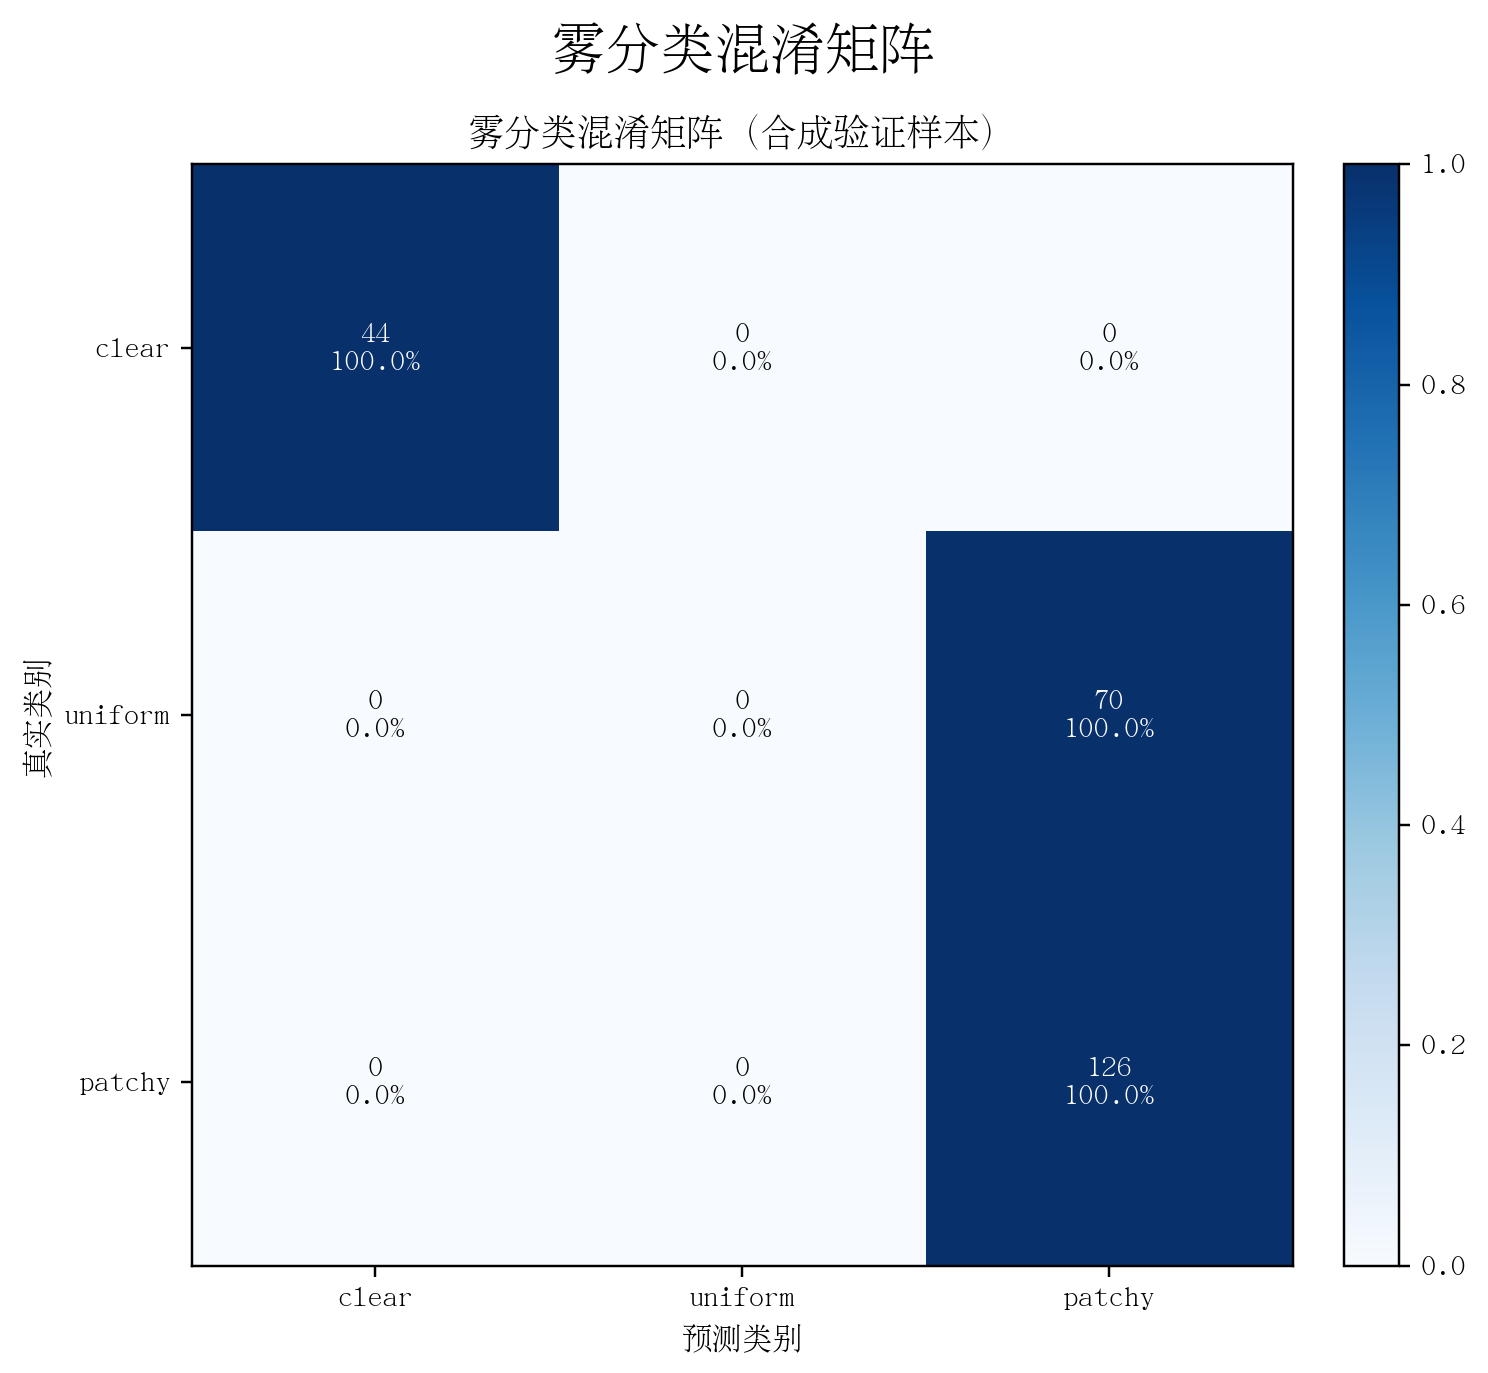
\includegraphics[width=0.72\textwidth]{fig_06_fog_class_confusion_matrix.png}
  \caption{雾分类混淆矩阵}
  \label{fig:fog_confusion_matrix}
\end{figure}

\begin{figure}[htbp]
  \centering
  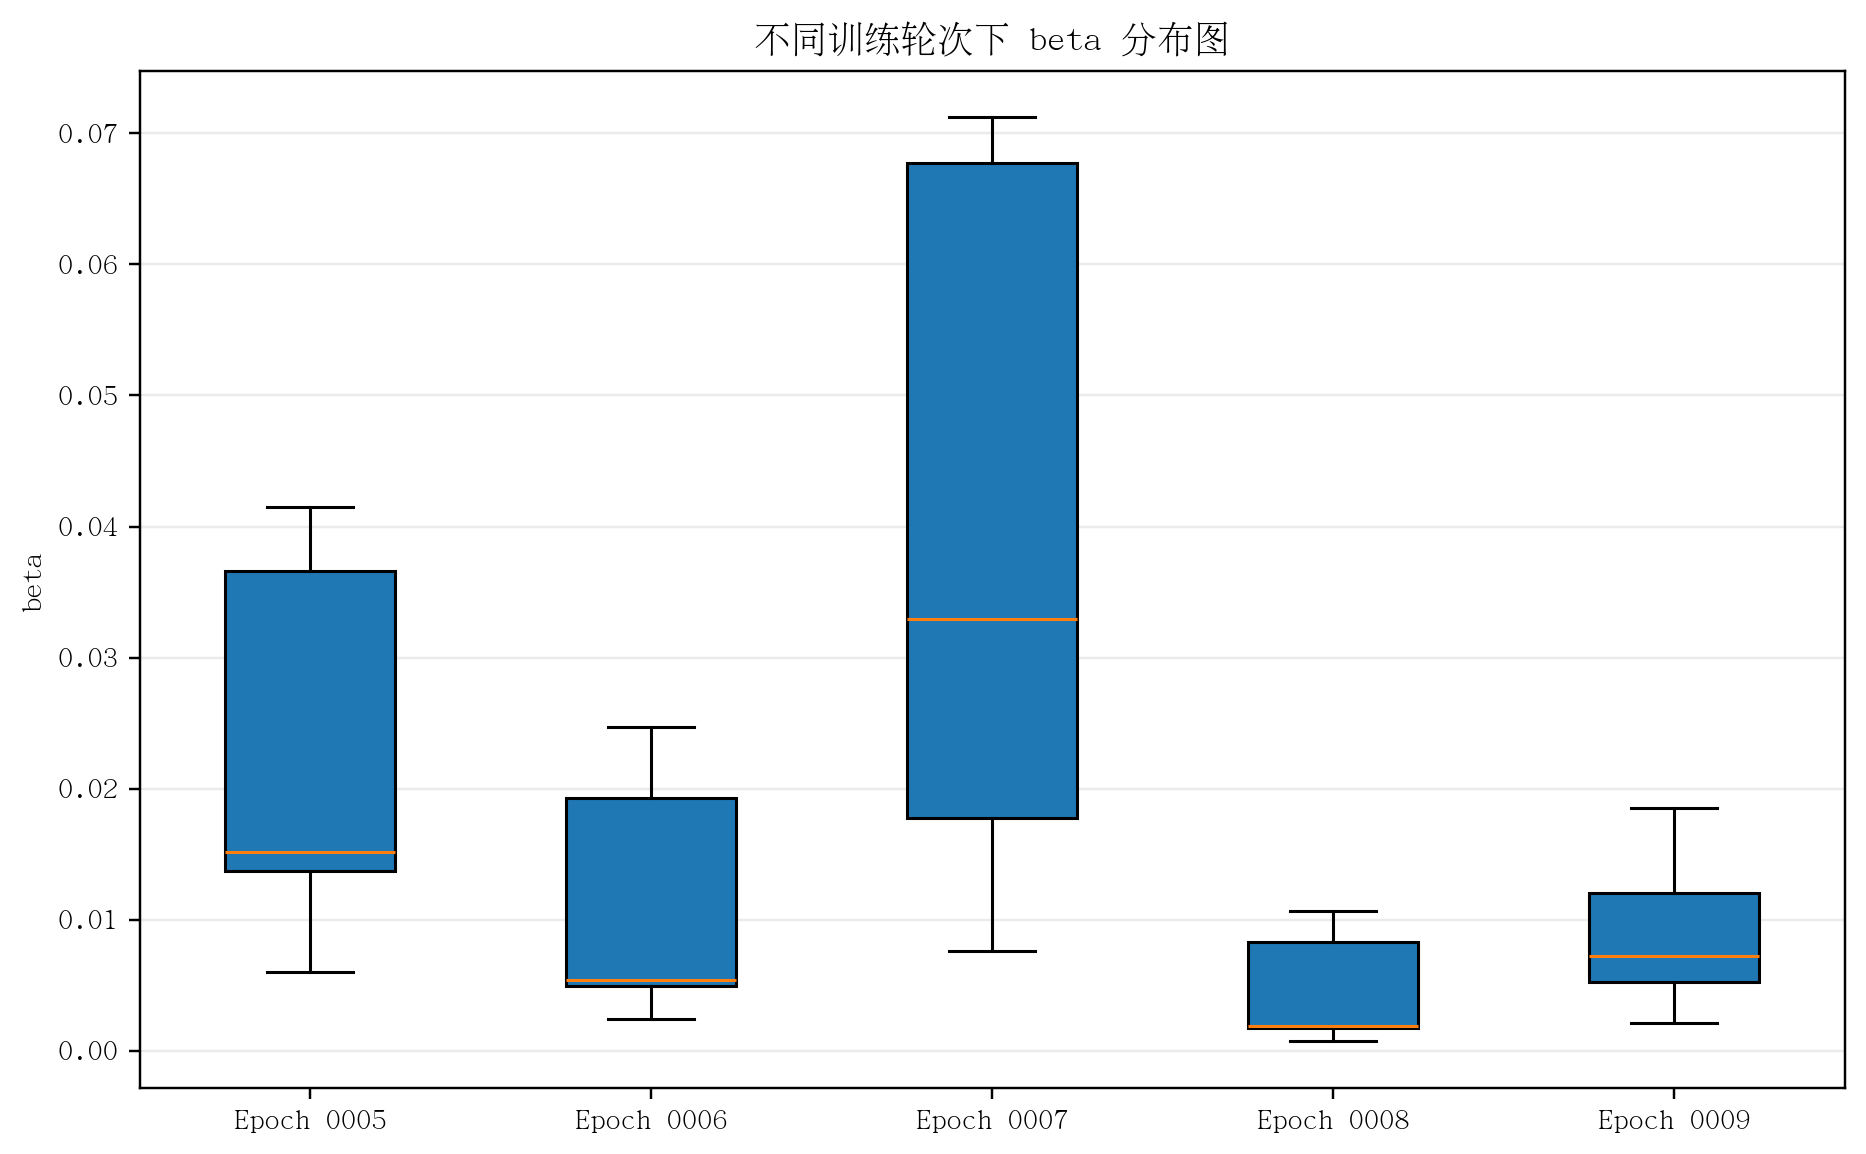
\includegraphics[width=0.82\textwidth]{fig_07_beta_distribution_by_epoch.png}
  \caption{不同训练轮次下 beta 分布图}
  \label{fig:beta_distribution}
\end{figure}

\section{真实雾视频结果}

为了观察正式雾权重在真实雾视频上的表现，本文首先对根目录中的 \code{gettyimages-1353950094-640_adpp.mp4} 做单视频路线评估。该视频分辨率为 768$\times$432，帧率为 30 FPS，在 \code{sample_stride = 5} 下共抽样 168 帧。

根据 \code{scripts/postprocess_fogfocus_full.py} 触发的路线评估结果，\code{fogfocus_full} 在该视频上的关键表现如表~\ref{tab:getty_real_fog_result} 所示。

\begin{table}[htbp]
  \centering
  \caption{正式 \code{fogfocus_full} 权重在真实雾视频上的结果}
  \label{tab:getty_real_fog_result}
  \small
  \begin{tabular}{@{}p{4.2cm}p{7.6cm}@{}}
    \toprule
    指标 & 数值 \\
    \midrule
    抽样帧数 & 168 \\
    mean beta & 0.06709 \\
    主导雾类别直方图 & \code{CLEAR: 2 / UNIFORM: 102 / PATCHY: 64} \\
    统一路线平均检测数/帧 & 0.685 \\
    统一路线非零检测帧占比 & 0.571 \\
    混合路线平均检测数/帧 & 1.768 \\
    推荐路线 & \code{hybrid} \\
    \bottomrule
  \end{tabular}
\end{table}

这一结果首先说明：\code{fogfocus_full} 已经明显打破默认统一模型在真实雾视频上“几乎全判 \code{clear}”的塌缩现象。换言之，雾分支的正式训练确实起到了作用。其次，它也同时说明：雾分支的改善并没有自动转化为检测分支的根本性提升。即使统一路线已经能稳定输出非 \code{clear} 主导的天气判断，其车辆检测表现仍弱于独立 \code{yolo11n.pt} 支撑的混合路线。

\begin{figure}[htbp]
  \centering
  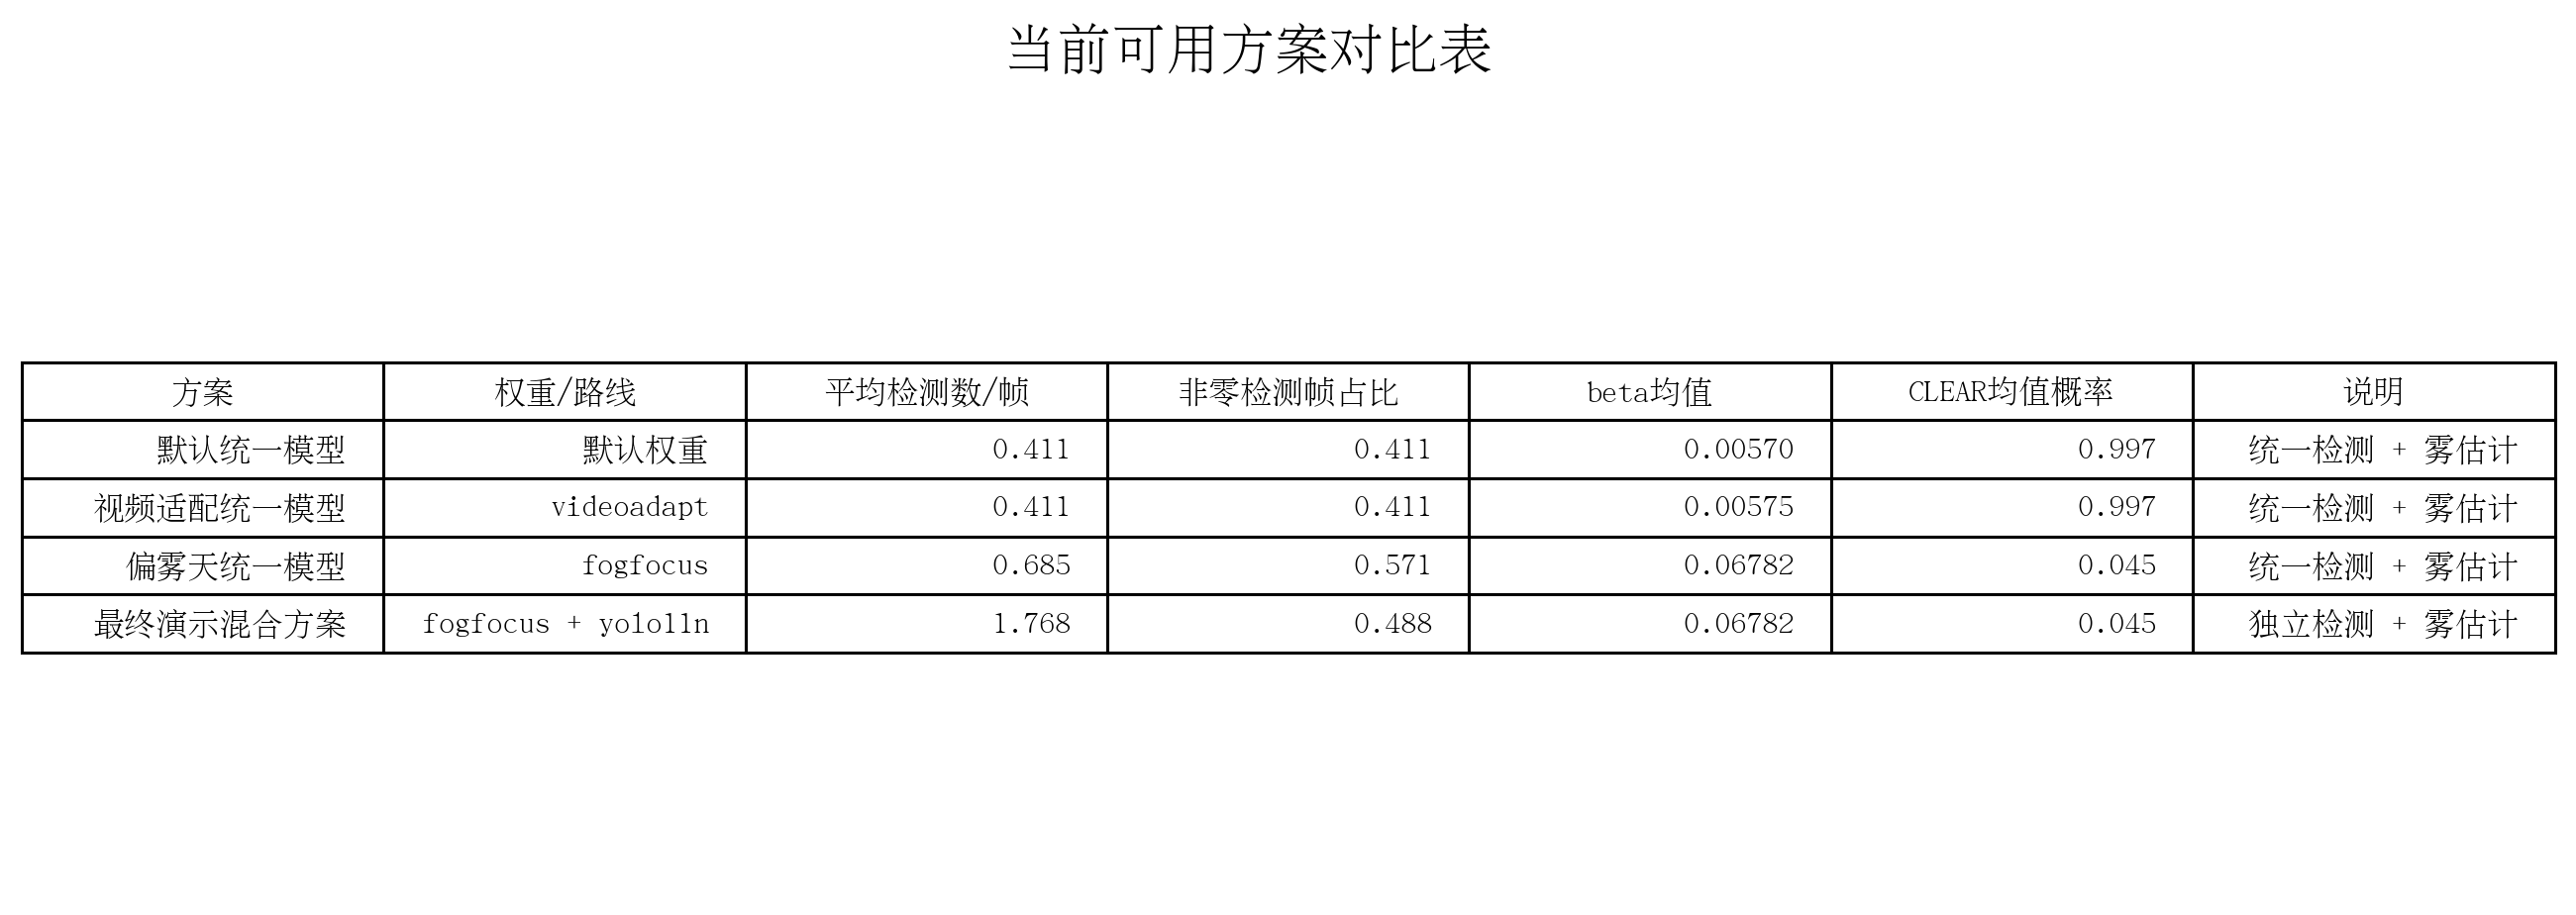
\includegraphics[width=\textwidth]{table_01_method_comparison.png}
  \caption{当前可用方案对比图}
  \label{fig:method_comparison}
\end{figure}

\section[benchmark\textunderscore{}v1 多模型结果]{benchmark\textunderscore{}v1 多模型结果}

\subsection{聚合结果}

仅看单段真实雾视频仍不足以支撑“论文正式模型选择”。为此，项目进一步使用 \code{benchmark_v1} 对 4 套 baseline 模型做了正式多模型基准评估。参与对比的模型分别是：

\begin{itemize}[leftmargin=2em]
\item \code{default_baseline}
\item \code{fogfocus}
\item \code{videoadapt}
\item \code{fogfocus_full}
\end{itemize}

聚合结果如表~\ref{tab:benchmark_v1_aggregate} 所示。

\begin{table}[htbp]
  \centering
  \caption{\code{benchmark_v1} 正式多模型聚合结果}
  \label{tab:benchmark_v1_aggregate}
  \scriptsize
  \resizebox{\textwidth}{!}{%
  \begin{tabular}{@{}lcccccc@{}}
    \toprule
    模型 & 统一均值/帧 & 非零帧占比 & 混合减统一 & beta 均值 & fog switch rate & beta abs delta \\
    \midrule
    \code{default_baseline} & 5.637 & 0.757 & 12.390 & 0.004624 & 0.000000 & 0.000141 \\
    \code{fogfocus} & 6.549 & 0.824 & 11.478 & 0.034476 & 0.007444 & 0.000999 \\
    \code{videoadapt} & 5.637 & 0.757 & 12.390 & 0.004711 & 0.000000 & 0.000138 \\
    \code{fogfocus_full} & 6.549 & 0.824 & 11.478 & 0.029682 & 0.032258 & 0.000906 \\
    \bottomrule
  \end{tabular}
  }
\end{table}

从中可以得到三点直接结论。

第一，\code{fogfocus} 与 \code{fogfocus_full} 在统一路线检测数和非零检测帧占比上并列当前最强，说明“偏雾天气头强化”确实能带来比默认统一模型更好的综合视频级表现。第二，\code{videoadapt} 虽然在单段目标视频适配上具有工程意义，但从当前 \code{benchmark_v1} 的 5 段视频正式结果看，它并未在统一路线检测指标上超越默认基线。第三，4 套模型的推荐路线全部仍然是 \code{hybrid}，这意味着截至当前工作区，最终工程演示路线并没有因为任何一版统一权重而被翻转。

值得注意的是，\code{fogfocus_full} 虽然与 \code{fogfocus} 在统一路线检测指标上并列，但它的 \code{weighted_beta_mean} 更低、\code{weighted_beta_abs_delta_mean} 略好，而 \code{weighted_dominant_switch_rate} 更高。这说明正式完整训练主要改变的是雾分支的分布特征和平滑性，而不是让统一检测分支完成质变。

\subsection{分视频结果}

进一步按视频展开 \code{fogfocus_full} 的结果，可得到表~\ref{tab:fogfocus_full_per_video}。

\begin{table}[htbp]
  \centering
  \caption{\code{fogfocus_full} 在 \code{benchmark_v1} 各视频上的表现}
  \label{tab:fogfocus_full_per_video}
  \small
  \begin{tabular}{@{}p{3.3cm}cccc@{}}
    \toprule
    视频 & 统一均值/帧 & 混合均值/帧 & 差值（hybrid-unified） & 主导雾类别 \\
    \midrule
    Getty 雾视频 & 0.685 & 1.768 & 1.083 & \code{UNIFORM FOG} \\
    稀疏车流对照 & 7.117 & 21.050 & 13.933 & \code{CLEAR} \\
    中等车流对照 & 5.983 & 29.300 & 23.317 & \code{CLEAR} \\
    较重车流对照 & 11.883 & 29.150 & 17.267 & \code{CLEAR} \\
    密集车流对照 & 17.633 & 38.133 & 20.500 & \code{CLEAR} \\
    \bottomrule
  \end{tabular}
\end{table}

这张表把统一模型当前的真正短板暴露得非常清楚：在真实雾视频上，统一路线和混合路线之间已经存在稳定差距；而在 4 段晴天对照视频片段上，这种差距进一步被放大。由此可见，当前统一模型的问题并不只是“雾头不够稳定”，更关键的是 \textbf{晴天交通视频中的检测能力仍然明显弱于独立 \code{yolo11n}}。

\section{UA-DETRAC 检测指标}

为了补足更标准的检测侧证据，本文新增实现了 \code{scripts/evaluate_uadetrac_detection_metrics.py}，在 UA-DETRAC 验证集上对若干关键权重做单类车辆检测评估。该脚本沿用论文正文一致的输入尺寸、letterbox 几何约定和验证划分规则，在清晰天气域上统计 Precision、Recall、mAP@0.5 和 mAP@0.5:0.95。结果如表~\ref{tab:uadetrac_standard_det_metrics} 所示。

\begin{table}[htbp]
  \centering
  \caption{UA-DETRAC 验证集上的标准检测指标}
  \label{tab:uadetrac_standard_det_metrics}
  \small
  \begin{tabular}{@{}p{3.6cm}ccccp{3.0cm}@{}}
    \toprule
    方法 & Precision & Recall & mAP@0.5 & mAP@0.5:0.95 & 说明 \\
    \midrule
    默认 unified 模型 & 0.8836 & 0.8038 & 0.8937 & 0.6570 & \code{outputs/Fog_Detection_Project/unified_model_best.pt} \\
    \code{fogfocus} 权重 & 0.8720 & 0.7700 & 0.8645 & 0.6204 & \code{outputs/Fog_Detection_Project_fogfocus/unified_model_best.pt} \\
    \code{fogfocus_full} 权重 & 0.8720 & 0.7700 & 0.8645 & 0.6204 & \code{outputs/Fog_Detection_Project_fogfocus_full/unified_model_best.pt} \\
    \code{yolo11n} 车辆基线 & 0.8077 & 0.7344 & 0.8102 & 0.5714 & 最终混合路线所使用的独立检测器 \\
    \bottomrule
  \end{tabular}
\end{table}

为使表~\ref{tab:uadetrac_standard_det_metrics} 的数值结果更具可读性，图~\ref{fig:detection_error_cases} 进一步给出了 \code{fogfocus_full} 权重在 UA-DETRAC 验证集上的一例典型漏检和一例典型误检。左图中，高亮框对应被漏检的车辆目标；右图中，高亮框对应高置信误检区域。可以看到，这些错误往往并非发生在目标完全不可见的场景，而是更容易出现在遮挡、透视形变、目标边界不完整或相邻车辆结构相互干扰的区域。

\begin{figure}[htbp]
  \centering
  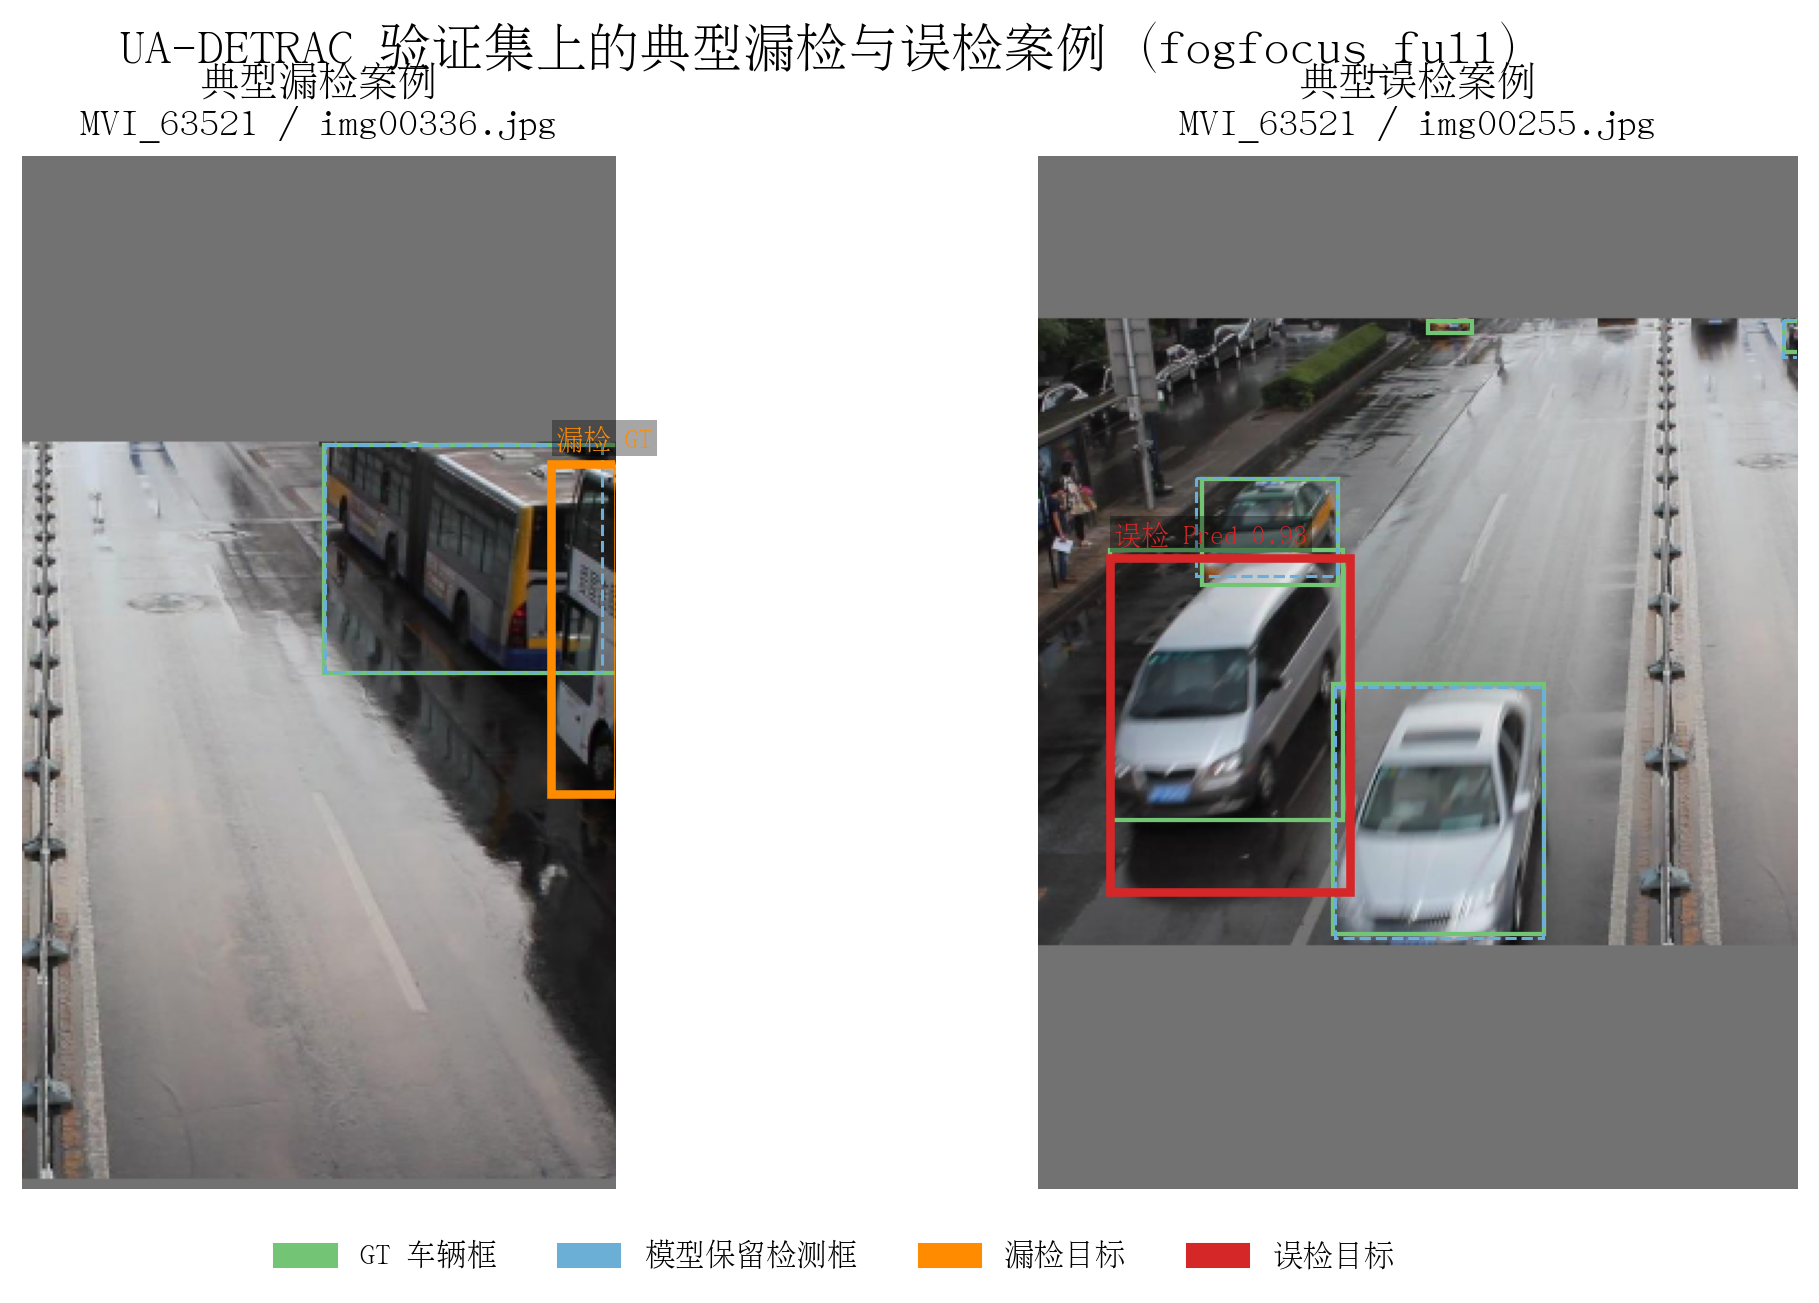
\includegraphics[width=0.96\textwidth]{fig_10_detection_error_cases.png}
  \caption{UA-DETRAC 验证集上的典型漏检与误检案例}
  \label{fig:detection_error_cases}
\end{figure}

表~\ref{tab:uadetrac_standard_det_metrics} 至少说明了三件事。

第一，若只看 UA-DETRAC 清晰天气验证集上的标准检测指标，默认 unified 模型实际上是当前表现最好的。这与其训练来源是一致的：默认 unified 检测分支直接在当前单类车辆任务上优化，因此在同域晴天验证集上取得最高 Precision、Recall 和 mAP 并不意外。

第二，\code{fogfocus} 与 \code{fogfocus_full} 的检测指标完全一致，这与当前训练策略严格对应。原因在于 \code{fogfocus_full} 正式训练阶段冻结了检测器并把 \code{DET_LOSS_WEIGHT} 设为 0，因此其正式训练主要改变的是雾分类头和 beta 回归头，而不是检测分支本身。于是，晴天验证集上的检测指标与 \code{fogfocus} 保持一致是合理现象，而不是统计误差。

第三，\code{yolo11n} 在 UA-DETRAC 晴天验证集上的标准检测指标反而低于经过单类任务适配的 unified 检测分支。这一点看似与前文的混合路线推荐结论相矛盾，但实则回答的是不同问题：UA-DETRAC 标准检测指标衡量的是“在同域清晰验证集上，检测器对单类车辆标注的拟合质量”；而 \code{benchmark_v1} 的路线评估衡量的是“在真实雾视频和少量晴天对照视频片段上，经过各自推理策略、阈值、时序过滤和可视化保留逻辑后，哪条完整路线更适合作为当前系统演示方案”。两类指标面向的问题不同，因此出现“标准检测表默认 unified 更强，但视频级推荐仍是 hybrid”的结果，并不冲突。

进一步从论文写作角度看，这张标准检测表的重要意义在于，它让本文不再只是依赖视频级现象判断检测分支的好坏，而是补上了一张更符合目标检测研究习惯的量化表。与此同时，它也迫使我们对当前系统做出更细致的分层判断：\textbf{默认 unified 在同域晴天车辆检测上并不弱；当前真正困难的，是如何把这种清晰天气检测能力与真实雾场景下的天气感知能力、视频级稳定性和时序过滤逻辑统一到一条更优的完整路线中。}

\section{检测回拉分支实验}

为了尝试修复上述短板，项目在 \code{fogfocus_full} 之后继续开展了三条检测能力回拉分支：\code{clearpreserve_pilot}、\code{detectorrecovery_pilot} 和 \code{cocohead_pilot}。它们的定位并不相同：

\begin{itemize}[leftmargin=2em]
\item \code{clearpreserve_pilot}：在保留雾任务的同时，通过清晰图检测损失辅助恢复检测能力；
\item \code{detectorrecovery_pilot}：进一步只做 clear 图检测恢复，观察“纯检测回拉”是否更有效；
\item \code{cocohead_pilot}：不再压缩为单类检测头，而是保留 COCO 80 类检测头结构。
\end{itemize}

这三条分支在正式候选模型基准评估中的聚合结果如表~\ref{tab:detector_recovery_branches} 所示。

\begin{table}[htbp]
  \centering
  \caption{三条检测能力回拉分支的候选 benchmark 结果}
  \label{tab:detector_recovery_branches}
  \scriptsize
  \resizebox{\textwidth}{!}{%
  \begin{tabular}{@{}lcccccc@{}}
    \toprule
    分支 & 统一均值/帧 & 非零帧占比 & 混合减统一 & beta 均值 & fog switch rate & 判定结果 \\
    \midrule
    \code{clearpreserve_pilot} & 5.645 & 0.723 & 12.382 & 0.0485 & 0.0720 & 未通过 \\
    \code{detectorrecovery_pilot} & 5.760 & 0.691 & 12.267 & 0.0536 & 0.0447 & 未通过 \\
    \code{cocohead_pilot} & 0.074 & 0.071 & 17.953 & 0.0494 & 0.0571 & 未通过 \\
    \bottomrule
  \end{tabular}
  }
\end{table}

需要特别强调的是，表中的“未通过”不是论文作者主观评价，而是由 \code{scripts/benchmark_candidate_model.py} 根据统一路线平均检测数、非零检测帧占比、fog 切换率和 beta 抖动等门槛自动给出的判定结论。三条分支全部未能通过门槛判定，说明当前问题并不能通过“临时补一轮检测损失”或“简单切换检测头模式”被快速修复。

进一步观察可以发现：

\begin{enumerate}[leftmargin=2.5em]
\item \code{clearpreserve_pilot} 的统一平均检测数与默认基线基本持平，但非零检测帧占比下降，且 fog 切换率明显恶化，说明它没有实现“检测回补而雾任务保持稳定”的预期。
\item \code{detectorrecovery_pilot} 在统一平均检测数上略高于 \code{clearpreserve_pilot}，但非零检测帧占比更差，说明“只做 clear 图检测恢复”同样未能解决根问题。
\item \code{cocohead_pilot} 则出现了最明显的失败：保留 COCO 80 类检测头并没有带来检测能力恢复，反而使统一路线的检测数量几乎崩塌。
\end{enumerate}

从研究视角看，这些失败分支并非负担，而是具有分析价值的结果。它们说明：统一模型当前的检测短板并不是某一个超参数或某一个头部形状选择就能轻易修复，而更可能与“真实雾域和合成雾域的差距”“单类检测头长期冻结后的表示退化”“统一模型在晴天对照视频片段上的检测表达不足”等更深层原因有关。也正因如此，论文最终应当保留这些失败结论，而不是只保留成功路线。

\section{静止误检治理实验}

\subsection{轨迹级指标}

为把“静止背景物体持续被误检成车辆”的问题从经验现象收口成可评估对象，项目在 \code{Route_Eval_temporal_smoke} 中加入了轨迹日志、逐帧过滤摘要和启发式静止误检指标。当前 5 段视频冒烟路线评估在 \code{sample_stride = 10}、\code{max_frames = 40} 下得到的聚合结果如表~\ref{tab:temporal_fp_metrics} 所示。

\begin{table}[htbp]
  \centering
  \caption{静止假车误检治理冒烟评估的聚合指标}
  \label{tab:temporal_fp_metrics}
  \small
  \begin{tabular}{@{}lcc@{}}
    \toprule
    指标 & 统一路线 & 混合路线 \\
    \midrule
    \code{heuristic_persistent_static_fp_per_min} & 29.35 & 58.70 \\
    \code{suppressed_heuristic_persistent_static_fp_per_min} & 29.35 & 48.91 \\
    \code{mean_confirmation_latency_frames} & 31.53 & 32.47 \\
    \bottomrule
  \end{tabular}
\end{table}

这些值不是带逐轨迹人工真值的严格误检率，但它们已经能够稳定回答两个问题：第一，当前静止误检现象确实存在，而且在混合路线中更严重；第二，时序过滤并不是“删掉所有低置信框”的粗暴后处理，而是以轨迹级形式显式记录了确认延迟、静止候选数量和已抑制静止候选数量。

\subsection{patch 复核与 negatives}

在当前工作区中，时序过滤器已经能够把被判为静止可疑或已抑制的轨迹导出为 patch。当前一轮冒烟测试共导出了 16 个 patch，其中统一路线 3 个、混合路线 13 个。随后，\code{scripts/build_static_fp_review_pack.py} 会基于置信度、运动强度、道路先验和外观概率，为这些 patch 赋予 \code{likely_false_positive}、\code{review_required} 和 \code{needs_careful_review} 等启发式标签。

在此基础上，项目又保守收口出一版 \code{Hard_Negatives_static_fp_v1}。当前该数据集中共有 4 个 bootstrap hard negatives，全部来自真实雾视频中的高置信非车辆误检。尽管规模很小，但这已经足以证明“轨迹日志导出 $\rightarrow$ patch 复核 $\rightarrow$ bootstrap negatives 收口”这条工程链路不是停留在文档层面的设想，而是已经形成真实产物。

\subsection{二次复核器}

基于上述 bootstrap negatives 和从 UA-DETRAC 中裁切得到的车辆正样本，当前项目训练了一版 \code{MobileNetV3_Small} 二分类复核器。其训练摘要显示：

\begin{itemize}[leftmargin=2em]
\item 车辆正样本数：96
\item bootstrap 负样本数：9
\item 最佳验证准确率：0.96875
\end{itemize}

更重要的是，当前工作区并不是只有“分类器训练成功”的离线结果，而是已经把这版权重回接到了 \code{TemporalVehicleFilter} 中。一次面向真实雾视频的二阶段复核冒烟评估显示，轨迹日志中已经明确出现 \code{appearance_non_vehicle} 作为抑制原因，且 \code{second_stage_classifier_enabled = True}、\code{init_error = None}。这说明二次复核器已经能够在真实推理链中实际生效，而不只是训练后孤立保存在某个目录中。

当然，就当前 1 段视频、40 个抽样帧的二阶段复核冒烟结果而言，还不足以严谨宣称“二次复核器已经显著降低静止误检率”。原因在于当前视频规模很小、阈值设置仍较保守，而且 per-minute 指标在超短视频上会被放大。更准确的结论应当是：\textbf{二次复核器的训练、加载、打分和回接路径已经打通，但其泛化收益仍需在更大视频集上继续验证。}

\section{结果讨论}

综合正式训练、正式基准评估和误检治理实验，可以得到以下判断。

第一，当前项目最稳固的成功点在于雾分支。无论从 \code{fogfocus_full} 的训练曲线、单段真实雾视频上的非 \code{clear} 主导结果，还是 5 段视频正式基准评估中 \code{fogfocus / fogfocus_full} 对默认基线的提升来看，雾分类与 beta 回归已经从“能跑”进入“可稳定输出、可做正式比较”的阶段。

第二，当前统一模型最明确的短板仍然是检测分支，尤其是在晴天对照视频片段上的车辆检测能力。正式基准评估与三条失败回拉分支都指向同一结论：这一短板不是某个临时微调脚本就能轻易修补的，因此当前最务实的系统路线仍然是“统一模型负责雾感知，独立 YOLO 负责车辆检测”的混合方案。

第三，项目的工程价值已经不再只体现在“有一个模型文件”。当前代码库已经形成了配置统一、训练可恢复、基准评估可复用、候选模型可门槛判定、静止误检可回灌的完整实验基础设施。对于毕业设计而言，这一点非常关键，因为它使论文不再只是展示一个静态结果，而是展示一个可持续迭代的工程研究框架。

\section{当前不足}

尽管论文主线已经能够和当前代码及实验产物保持一致，但从严格研究角度看，仍存在以下不足。

\begin{enumerate}[leftmargin=2.5em]
\item \textbf{真实雾视频覆盖仍然不足。} 当前 \code{benchmark_v1} 虽然已经从“单视频模板”扩展到 5 段有效视频资产，但其中真实雾视频仍只有 1 段，其余 4 段为晴天对照视频片段。
\item \textbf{真实雾域上的标注型检测指标仍然缺失。} 当前新增的标准检测表已经覆盖 UA-DETRAC 晴天验证集，但真实雾视频仍缺少逐框人工标注，因此无法在雾域上给出同等严格的 mAP 对照。
\item \textbf{beta 仍缺少外部物理标定。} 当前 beta 具有稳定的相对意义，但尚未与真实能见度仪或气象站观测建立严格对应关系。
\item \textbf{二次复核器数据规模较小。} 当前 bootstrap negatives 的规模只足以证明链路可行，尚不足以支撑更强泛化结论。
\item \textbf{系统性消融仍待完善。} 后续可围绕是否使用深度、是否加入 \code{patchy} 模式、是否接入时序过滤和二次复核器等因素开展对照实验。
\end{enumerate}

因此，后续更严格的补充实验应优先围绕以下三类展开：其一，在 UA-DETRAC 验证集上补充标准检测指标；其二，在更多真实雾视频上扩展 \code{benchmark_v2}；其三，对静止误检治理链做成体系的消融实验，而不是只保留冒烟路线证据。

\section{应用分析}

若结合陕西交通运输部门当前的运行管理现状来看，本文项目的应用价值可以从“可接入、可解释、可联动、可渐进部署”四个维度进一步理解。

首先，从“可接入”角度看，陕西省交通运输系统并不缺监控和监测基础，而是更需要让既有视频资源具备更强的场景理解能力。陕西省交通运输厅公开预算资料中已明确列出“陕西省高速公路网运行监测能力提升”项目，说明省级层面已持续投入路网运行监测。与此同时，陕西省高速公路监测预警系统建设（第一批）覆盖 18 家路段分公司、142 处风险点，表明监测预警建设已经从理念阶段进入实施阶段\cite{shaanxiBudget2025,shaanxiRiskProject2025}。对于本文项目而言，这意味着它不需要重新建设前端感知设施，而可以优先以软件方式接入既有监控视频流，在现有体系中增加雾分类、beta、车辆检测三类结果。

其次，从“可解释”角度看，陕西交通部门在实际运行中需要的不只是一个黑盒判定，而是能够参与值班研判和协同处置的解释型结果。公路运行周报机制表明，陕西省公路局会持续接收并转发气象灾害预警信息，并结合重点线路交通量开展路网研判；这类业务并不是简单地看“是否有雾”，而是要回答“雾有多重、车流有多大、是否需要限速、是否需要分流、是否要提前预置力量”等更具体的问题\cite{shaanxiWeekly2025,shaanxiWhitepaper2024}。本文项目的雾类型、beta 连续值、车辆检测数量与动态阈值联动结果，恰好能对应这种解释需求：既可为值班人员提供直观依据，也可为后续等级化策略设计提供参数基础。

再次，从“可联动”角度看，陕西已经在恶劣天气处置方面形成较强的部门协同意识。2025 年 12 月的陕渝省际高速公路低温雨雪冰冻天气暨隧道突发事件应急演练，完整展示了监测预警、会商研判、力量预置、交通管控和救援保障等环节的联动过程\cite{shaanxiEmergency2025}。这说明，真正有价值的系统并不是只在视频里画几个框，而是要能够成为联动链条中的一环。本文项目若部署在陕西场景中，其输出结果最适合作为“一路多方”会商前端的视觉补充信息：例如把“uniform / patchy + beta + 当前检测数 + 代表帧截图”同步推送给值班调度、路政、养护、收费和交警协同体系，用于辅助判定风险等级和控制策略。

最后，从“可渐进部署”角度看，当前正式基准评估的结论与陕西场景的工程现实较为一致。当前离线对比已经反复表明：统一模型在雾感知层面已经有明显进展，但在车辆检测层面仍弱于混合路线。因此，若面向陕西交通部门开展原型验证，最务实的选择并不是强行坚持“一个模型做完所有事”，而是优先采用“正式雾任务权重 + 独立 YOLO 检测”的混合方案。这样做更符合政府部门信息化项目的落地逻辑：先保证结果可靠可用，再逐步推进统一模型替代，而不是为了模型结构完整性牺牲当前可交付性。

综合来看，本文项目与陕西交通部门现状的结合，不应停留在论文背景层面的“举例说明”，而应进一步明确为一种可落地的应用路径：以既有监控视频为输入，以雾风险识别为核心，以协同联动和分级处置为目标，在陕西现有监测预警和路网运行体系中形成一个可逐步接入、逐步验证、逐步扩展的智能感知模块。

\section{本章小结}

本章围绕训练结果、视频级基准评估、标准检测指标、误差案例以及静止误检治理链，对当前工作区中的实验产物进行了系统分析。结果表明：一方面，\code{fogfocus_full} 已经能够作为正式论文中的雾任务参考权重，说明统一模型的雾分类与 beta 回归分支具备较稳定的训练与推理表现；另一方面，正式基准评估又明确暴露出统一模型在晴天对照视频片段上的检测短板，使“正式雾任务权重 + 独立 YOLO 检测”的混合路线成为当前阶段最务实的工程方案。同时，静止误检治理链和二次复核器训练结果说明，项目已经具备从视频级误检现象出发，逐步形成可记录、可复核、可回灌闭环的工程能力。这些结论共同构成了全文总结与后续展望的实验依据。

\chapter{结论与展望}

本文围绕高速公路团雾监测这一典型低能见度智能交通问题，提出并实现了一种基于深度估计与多任务学习的统一监测方法。针对真实团雾样本稀缺、浓度标签难以获取、固定监控视频场景与自动驾驶数据差异明显等问题，本文选择以 UA-DETRAC 清晰交通数据为基础，通过 MiDaS\_small 预计算深度缓存，构建基于大气散射模型的在线造雾机制，在训练阶段动态生成 clear、uniform、patchy 三类天气样本，并进一步设计统一多任务模型同时完成车辆检测、雾类型分类和 beta 浓度回归。与单一任务研究相比，本文方法更贴近高速公路监控场景下的真实业务需求。

在工程实现方面，本文完成了从数据准备、训练、验证、视频推理到导出与量化路径的完整闭环。当前工作区已经能够稳定读取原始数据、补齐深度缓存、执行联合训练并输出模型权重；推理脚本能够在视频中显示雾类别、beta 数值、车辆检测结果和动态阈值控制效果；混合推理脚本则进一步解决了早期统一模型在真实雾视频上车辆检测能力不足的问题，并构建了带中文标题、刻度条和分级标签的雾浓度分布图小地图，从而显著提升了系统演示的完整性与可解释性。

从研究结论看，本文工作至少说明了以下几点。第一，在高速公路固定监控视频场景中，利用单目深度估计和在线物理造雾构造多任务训练监督是可行的。第二，将车辆检测、雾分类和雾浓度回归整合为统一多任务模型具有合理性，并已在工程上打通训练与推理主链。第三，基于 beta 的时间平滑和检测阈值联动，为天气感知参与业务决策提供了初步可执行路径。第四，即使统一模型尚在持续优化，通过混合推理也可以较快形成可视化系统原型，为论文验证和后续工程迭代争取时间。

当然，本文仍处于毕业设计原型系统阶段，尚有若干值得深入推进的方向。未来工作可从以下几个方面展开。

首先，应继续强化真实雾域适应能力。一种可行做法是在当前在线造雾训练框架基础上，引入少量真实雾视频做有监督或半监督微调，以缩小合成雾与真实雾之间的域差距。

其次，可将当前的全局 beta 回归扩展为空间雾浓度预测。若能设计一个密集回归分支输出逐像素或分块级雾浓度图，则右下角的小地图就能够从“解释增强近似图”升级为真正的模型预测结果。

再次，可引入更直接的能见度标定数据。如果后续能够获得路侧气象站、能见度仪、激光雷达或人工等级标注数据，就可以将 beta 与真实能见度建立更明确对应关系，增强结果的物理意义。

最后，在部署层面，本文已预留 QAT、INT8 和 ONNX 路径，未来可以进一步围绕 Jetson 或路侧边缘设备开展推理速度、功耗、时延和稳定性测试，使该系统真正走向“可部署、可维护、可联动”的交通气象智能监测原型。

若进一步结合陕西省交通运输行业现状，未来工作还可以围绕三个更具体的方向推进。第一，面向陕西交控集团和省级路网运行部门的既有监测预警项目，探索将本文的视频雾风险识别能力以插件方式接入现有风险点工程与值班调度流程；第二，围绕西安绕城、新机场线、连霍高速关中段和陕南山区桥隧通道，分别构建“高流量平原场景”和“高风险山地场景”两类验证样板，比较不同区域的雾特征差异与部署重点；第三，结合陕西交通部门已经形成的气象预警转发、路网周报和省际应急演练机制，进一步把模型输出从单纯的视频可视化结果提升为可直接进入限速诱导、情报板发布和会商研判的结构化信息。若这些工作能够继续推进，本文项目在陕西场景中的应用价值将不仅体现为一套毕业设计原型，而有望成为面向实际行业系统的小型智能模块。

总的来说，本文在高速公路团雾监测这一具有明显现实意义的问题上，完成了一套从理论方法到工程系统的完整探索。虽然仍有大量细节有待完善，但其方法框架、代码实现和可视化闭环已经具备较强的继续扩展价值，可为毕业设计终稿、后续论文发表以及实际道路监测应用提供坚实基础。


\chapter*{参考文献与资料链接}
\addcontentsline{toc}{chapter}{参考文献与资料链接}
\thispagestyle{plain}

\begin{quote}
注：以下文献与资料按“官方数据/标准优先、近两年论文优先、再补充经典基础文献”的原则整理。因本稿为初稿，参考文献格式后续可按学校模板统一调整。

\end{quote}

\section{官方统计数据、标准与行业资料}

\begin{enumerate}[leftmargin=2.5em]
\item 国家统计局. 《中华人民共和国 2025 年国民经济和社会发展统计公报》, 2026-02-28. \\
  链接：\url{https://www.stats.gov.cn/sj/zxfb/202602/t20260228_1958817.html}
\item 国家统计局. 《中华人民共和国 2024 年国民经济和社会发展统计公报》, 2025-02-28. \\
  链接：\url{https://www.stats.gov.cn/sj/zxfb/202502/t20250228_1958817.html}
\item 交通运输部. 《2024 年交通运输行业发展统计公报》, 2025-06-13. \\
  链接：\url{https://www.gov.cn/lianbo/bumen/202506/content_7027415.htm}
\item 国家统计局. 2025 年统计公报中有关汽车保有量与新能源汽车数据的公开信息检索页。 \\
  链接：\url{https://www.stats.gov.cn/sj/zxfb/202602/t20260228_1958817.html}
\item 中国气象局. QX/T 729—2024《高速公路交通安全管控天气风险预警等级》. \\
  链接：\url{https://www.cma.gov.cn/zfxxgk/gknr/flfgbz/bz/202404/t20240424_6223734.html}
\item 中国气象局. QX/T 808—2025《高速公路雾天视频图像能见度等级识别技术规范》, 2026-01-24 发布。 \\
  链接：\url{https://www.cma.gov.cn/zfxxgk/gknr/flfgbz/bz/202601/t20260124_6824607.html}
\item 美国联邦公路管理局（FHWA）. Road Weather Management Program: Weather Events and Their Impact on Roads. \\
  链接：\url{https://ops.fhwa.dot.gov/weather/q1_roadimpact.htm}
\item 美国联邦公路管理局（FHWA）. Road Weather Spotlight: Impact of Fog-Related Crashes. \\
  链接：\url{https://highways.dot.gov/public-roads/mayjune-1998/road-weather-spotlight-impact-fog-related-crashes}
\item 世界卫生组织（WHO）. Road traffic injuries factsheet. \\
  链接：\url{https://www.who.int/news-room/fact-sheets/detail/road-traffic-injuries}
\item 中国气象局. 2025 年试点发布高速公路浓雾和道路结冰风险地图等交通气象信息。 \\
  链接：\url{https://www.cma.gov.cn/2011xwzx/2011xztbd/2025nzt/2025nqxxmhwcxgzt/202501/t20250131_6838123.html}
\item 中国气象局. 公路交通灾害高影响路段致灾因子阈值相关技术资料。 \\
  链接：\url{https://www.cma.gov.cn/2011xzt/2024zt/20240109/2024010903/202410/t20241022_6640415.html}
\end{enumerate}

\section{近两年国外相关论文与综述}

\begin{enumerate}[leftmargin=2.5em]
\item \emph{Clear Roads, Clear Vision: Advancements in Multi-Weather Restoration for Smart Transportation}, 2025. \\
  链接：\url{https://arxiv.org/abs/2511.20865}
\item \emph{Estimating Fog Parameters from a Sequence of Stereo Images}, 2025. \\
  检索链接：\url{https://pubmed.ncbi.nlm.nih.gov/40540383/}
\item \emph{ADAM-Dehaze: Adaptive Multi-Scale Frequency-Aware Transformer and Attention Fusion Network for Single Image Dehazing}, 2025. \\
  链接：\url{https://arxiv.org/abs/2509.02217}
\item \emph{From Fog to Failure: Evaluating Weather-Agnostic Perception in Autonomous Vehicles}, 2025. \\
  链接：\url{https://arxiv.org/abs/2503.23504}
\item \emph{Defog YOLO for road object detection in foggy weather}, 2024. \\
  链接：\url{https://academic.oup.com/tse/article/8/2/tdae009/7637460}
\item \emph{Dehazing \& Reasoning YOLO: A real-time object detector for foggy driving scenes}, 2024. \\
  检索链接：\url{https://www.sciencedirect.com/science/article/pii/S0031320324002765}
\item \emph{Robust ADAS: Weather-Robust Object Detection Benchmarking and Analysis}, 2025. \\
  链接：\url{https://arxiv.org/abs/2505.10334}
\item \emph{WARLearn: Weather-Adaptive Representation Learning for Adverse Driving Perception}, 2025. \\
  链接：\url{https://arxiv.org/abs/2504.13758}
\item \emph{Fog-YOLO: A Real-Time Object Detector for Foggy Autonomous Driving Scenarios}, 2026. \\
  检索链接：\url{https://www.mdpi.com/2076-3417/16/4/1759}
\item \emph{Improved DeepSORT-Based Object Tracking in Foggy Weather for Intelligent Vehicles}, 2024. \\
  检索链接：\url{https://pmc.ncbi.nlm.nih.gov/articles/PMC11280926/}
\end{enumerate}

\section{近两年国内相关论文与研究资料}

\begin{enumerate}[leftmargin=2.5em]
\item 孙啸，等. 《雾天条件下交通气象预警阈值探究》, 《中国交通信息化》, 2024(6). \\
  检索链接：\url{https://d.wanfangdata.com.cn/periodical/zgjtxxcy202406014}
\item 邢万勇，等. 《大模型在高速公路事件检测中的应用探索》, 《中国交通信息化》, 2024(6). \\
  检索链接：\url{https://d.wanfangdata.com.cn/periodical/zgjtxxcy202406016}
\item 《基于 CycleGAN 的无监督图像去雾网络》, 2025. \\
  检索链接：\url{https://sns.wanfangdata.com.cn/sns/perio/dlhsdxxb/2025/3?perioId=dlhsdxxb_2025_3}
\item 《结合特征增强注意力的混合卷积去雾网络》, 2025. \\
  检索链接：\url{https://sns.wanfangdata.com.cn/sns/perio/xdjsk/2025/23?perioId=xdjsk_2025_23}
\item \emph{UMT-HPLA: 半监督雾天跨域目标检测模型}, 2025. \\
  检索链接：\url{https://www.jos.org.cn/josen/article/abstract/7014?st=search}
\item 《我国公路交通气象研究与业务进展》, 交通运输领域气象服务相关综述资料。 \\
  检索链接：\url{https://www.researching.cn/articles/OJ753aaf3b03cd61b2}
\end{enumerate}

\section{基础理论与数据集支撑文献}

\begin{enumerate}[leftmargin=2.5em]
\item Cordts M, et al. Cityscapes Dataset. \\
  链接：\url{https://www.cityscapes-dataset.com/}
\item Wen L, et al. UA-DETRAC: A new benchmark and protocol for multi-object detection and tracking. \\
  链接：\url{https://detrac-db.rit.albany.edu/}
\item Ranftl R, et al. MiDaS / Vision Transformers for Robust Monocular Depth Estimation. \\
  链接：\url{https://github.com/isl-org/MiDaS}
\item Koschmieder H. Theory of atmospheric scattering and visibility. \\
  经典理论文献，可在后续终稿中按学校模板补全书目信息。
\item Ultralytics. YOLO official documentation and implementation resources. \\
  链接：\url{https://docs.ultralytics.com/}
\item PyTorch Official Documentation. \\
  链接：\url{https://pytorch.org/docs/stable/index.html}
\end{enumerate}

\section{陕西省交通运输与公路运行监测相关资料}

\begin{enumerate}[leftmargin=2.5em]
\item 陕西省交通运输厅. 《2026年陕西省交通运输工作会议召开》, 2026-01-26. \\
  链接：\url{https://jtyst.shaanxi.gov.cn/sy/jdtp/202601/t20260126_3607783.html}
\item 陕西省交通运输厅. 《2026年全省公路工作会议暨公路行业安全生产第一次会议召开》, 2026-01-29. \\
  链接：\url{https://jtyst.shaanxi.gov.cn/sy/bmdt/202601/t20260129_3609067.html}
\item 陕西省交通运输厅. 《2025年高速公路监测预警系统建设（第一批）招标公告》, 2025-09-02. \\
  链接：\url{https://jtyst.shaanxi.gov.cn/glj/scgl/zbgg/202509/t20250902_3561698.html}
\item 陕西省交通运输厅. 《路网运行情况周报（2025年11月24日至11月30日）》, 2025-12-01. \\
  链接：\url{https://jtyst.shaanxi.gov.cn/glj/sy/lwyxdt/202512/t20251201_3590825.html}
\item 陕西省交通运输厅. 《陕西省干线公路网运行情况周报（2026年1月5日至1月11日）》, 2026-01-13. \\
  链接：\url{https://jtyst.shaanxi.gov.cn/glj/sy/lwyxdt/202601/t20260113_3604575.html}
\item 陕西省交通运输厅. 《陕渝砺兵 雪战通衢——2025年陕渝省际高速公路低温雨雪冰冻天气暨隧道突发事件应急演练举行》, 2025-12-16. \\
  链接：\url{https://jtyst.shaanxi.gov.cn/sy/bmdt/202512/t20251216_3596231.html}
\item 陕西省交通运输厅. 《〈2024年陕西省公路网运行白皮书〉发布》, 2025-08-14. \\
  链接：\url{https://jtyst.shaanxi.gov.cn/sy/bmdt/202508/t20250814_3554745.html}
\item 陕西省交通运输厅. 《2025年部门预算公开说明》, 2025-03-13. \\
  链接：\url{https://jtyst.shaanxi.gov.cn/zfxxgk/fdzdgknr/ysjs/202502/P020250313578082891523.pdf}
\end{enumerate}

\appendix
\chapter{核心实现与复现实验说明}

为便于后续复核、扩展和工程复现，本附录对本文系统的主要文件组织、核心脚本和典型实验命令进行说明。附录内容不重复正文中的算法推导和实验分析，仅作为论文对应工程实现的补充材料。

\section{项目主要文件组织}

本文系统采用数据处理、模型训练、推理部署和论文材料相互分离的组织方式，主要目录如下。

\begin{enumerate}[leftmargin=2.5em]
\item \code{src/}：系统核心源码目录，包含配置读取、统一多任务模型、训练流程、推理流程、模型导出和时序过滤等实现。
\item \code{scripts/}：实验与数据处理脚本目录，包含数据检查、深度缓存预计算、候选模型评估、视频基准测试、论文图表生成和误检样本挖掘等工具。
\item \code{configs/}：实验配置文件目录，用于保存模型训练、候选评估和视频基准测试所需的参数。
\item \code{docs/experiments/}：实验记录与结果整理目录，用于保存不同训练分支、候选模型和基准评估的文字记录。
\item \code{overleaf_thesis/}：论文 LaTeX 工程目录，包含西安电子科技大学本科毕业设计论文模板、正文、参考文献、图表和最终 PDF。
\end{enumerate}

\section{核心源码文件说明}

系统实现中与论文方法直接相关的核心文件包括：

\begin{enumerate}[leftmargin=2.5em]
\item \code{src/model/unified_model.py}：定义车辆检测、雾类型分类和 beta 回归统一建模结构，是本文多任务模型的核心实现。
\item \code{src/train.py}：实现训练主流程，包括数据加载、在线造雾、多任务损失计算、混合精度训练、checkpoint 保存与续训。
\item \code{src/inference.py}：实现单帧和视频推理所需的预处理、模型前向、检测结果后处理和雾状态输出。
\item \code{src/temporal_vehicle_filter.py}：实现轨迹级时序过滤，用于抑制固定监控视频中持续出现的静止假车误检。
\item \code{src/export.py}：提供模型导出接口，为后续 ONNX、TensorRT 和边缘端部署预留工程路径。
\end{enumerate}

\section{主要实验脚本说明}

本文实验过程中使用的主要脚本包括：

\begin{enumerate}[leftmargin=2.5em]
\item \code{scripts/check_dataset.py}：检查数据集路径、图像文件、标注文件和基础统计信息。
\item \code{scripts/precompute_depth_cache.py}：调用单目深度估计模型预计算深度缓存，降低训练阶段重复推理开销。
\item \code{scripts/smoke_test.py}：执行训练前冒烟测试，验证数据读取、模型前向、损失计算和反向传播链路是否正常。
\item \code{scripts/evaluate_uadetrac_detection_metrics.py}：在 UA-DETRAC 验证集上计算车辆检测相关指标。
\item \code{scripts/run_multi_model_benchmark.py}：对多个候选模型和多段视频执行统一基准评估。
\item \code{scripts/hybrid_fog_vehicle_infer.py}：实现“统一模型雾估计 + 独立 YOLO 车辆检测”的混合推理路线。
\item \code{scripts/build_detection_error_case_figure.py}：生成论文中用于误差案例分析的可视化图。
\end{enumerate}

\section{典型复现实验命令}

在依赖环境和数据路径配置完成后，可按如下流程复现本文主要实验链路。

\begin{enumerate}[leftmargin=2.5em]
\item 数据集检查：
\code{python scripts/check_dataset.py}
\item 深度缓存预计算：
\code{python scripts/precompute_depth_cache.py}
\item 训练前冒烟测试：
\code{python scripts/smoke_test.py}
\item 统一多任务模型训练：
\code{python -m src.train}
\item 候选模型视频基准评估：
\code{python scripts/run_multi_model_benchmark.py}
\item 混合推理视频生成：
\code{python scripts/hybrid_fog_vehicle_infer.py}
\item 论文 LaTeX 编译：
\code{latexmk -xelatex -interaction=nonstopmode -halt-on-error main.tex}
\end{enumerate}

实际复现实验时，应根据本机数据集位置、权重文件路径和输出目录调整配置文件中的路径参数。若只进行论文编译，则无需运行模型训练脚本，只需保证 \code{overleaf_thesis/} 目录中的模板文件、章节文件、参考文献文件和图像文件完整即可。


\end{document}
